%!TEX root = ./main.tex
%
% This file is part of the i10 thesis template developed and used by the
% Media Computing Group at RWTH Aachen University.
% The current version of this template can be obtained at
% <http://www.media.informatik.rwth-aachen.de/karrer.html>.

\documentclass[11pt, a4paper, titlepage]{book}

% ! ACHTUNG !
% Nach dem ersten LaTeX durchlauf auf der Kommandozeile
% makeindex -s main.ist main.idx
% ausf�hren, sonst wird der Index nicht so sch�n formatiert.
% Leider macht TeXShop den makeindex Aufruf nur ohne Parameter.

% !ATTENTION!
% After running LaTeX for the first time using this template call
% makeindex -s main.ist main.idx
% to get the correct formatting for the index.

%Pakete und eigene Befehle - am besten durchlesen!
%Includes all neccessary packets and contains some useful commands - read this file!
%!TEX root = ./main.tex

% This file is part of the i10 thesis template developed and used by the
% Media Computing Group at RWTH Aachen University.
% The current version of this template can be obtained at
% <http://www.media.informatik.rwth-aachen.de/karrer.html>.



%-----------------------------------------------------------------------------------------------------------------------------------------
% Befehle
% commands
%-----------------------------------------------------------------------------------------------------------------------------------------

%----------------------------------------------------------------------------------
% \myBigFigure	[ LABEL_PREFIX (optional) ]
%				{ FILENAME (without extension) }
%				{ CAPTION TEXT }
%				{ SHORT VERSION OF CAPTION TEXT }
%
%Bild wird in kompletter Breite gesetzt, die Kurzversion der Bildunterschrift erscheint im Abbildungsverzeichnis
%picture using full width of the page, the short caption is what appears in the list of figures index

%----------------------------------------------------------------------------------
% \myFrameBigFigure	[ LABEL_PREFIX (optional) ]
%					{ FILENAME (without extension) }
%					{ CAPTION TEXT }
%					{ SHORT VERSION OF CAPTION TEXT }
%
%Bild wird in kompletter Breite gesetzt und eingerahmt, die Kurzversion der Bildunterschrift erscheint im Abbildungsverzeichnis
%picture with frame using the full width of the page, the short caption is what appears in the list of figures index

%----------------------------------------------------------------------------------
% \myHUGEFigure	[ LABEL_PREFIX (optional) ]
%				{ FILENAME (without extension) }
%				{ CAPTION TEXT }
%				{ SHORT VERSION OF CAPTION TEXT }
%
%Bild wird rotiert und quer in kompletter Breite gesetzt, die Kurzversion der Bildunterschrift erscheint im Abbildungsverzeichnis
%landscape picture using the full width of the rotated page, the short caption is what appears in the list of figures index

%----------------------------------------------------------------------------------
% \myFigure	[ LABEL_PREFIX (optional) ]
%			{ FILENAME (without extension) }
%			{ CAPTION TEXT }
%			{ SHORT VERSION OF CAPTION TEXT }
%
%Bild wird in der Breite der textspalte gesetzt, die Kurzversion der Bildunterschrift erscheint im Abbildungsverzeichnis
%picture using the width of the text column, the short caption is what appears in the list of figures index

%----------------------------------------------------------------------------------
% \myImgRef	[ LABEL_PREFIX (optional) ]
%			{ LABEL OF THE IMAGE }
%
%referenziert das angegebene Bild
%reference to an image

%----------------------------------------------------------------------------------
% \myBigTable	{ YOUR TABULAR DEFINITION }
%			{ CAPTION TEXT }
%			{ TABLE_LABLE }
%
%Tabelle wird in kompletter Breite gesetzt
%table using the full width of the page

%----------------------------------------------------------------------------------
% \myTable	{ YOUR TABULAR DEFINITION }
%			{ CAPTION TEXT }
%			{ TABLE_LABLE }
%
%Tabelle wird in der Breite der Textspalte gesetzt
%table using the width of the text column

%----------------------------------------------------------------------------------
% \myTxtRef	{ LABLE }
%
%Referenz auf Kapitel oder Abschnitte - gibt nummer und namen aus, z.B.: 5.3---"Yaddahyaddah"
%references chapters or sections, outputs number and title, e.g., 5.3---"Yaddahyaddah"

%----------------------------------------------------------------------------------
% \myUnderscore
%
%Setzt einen "sch�nen" Unterstrich f�r URLs
%typesets a 'nice' underscore for URLs

%----------------------------------------------------------------------------------
%\myTilde
%
%Setzt eine "sch�ne" Tilde f�r URLs
%typesets a 'nice' tilde for URLs

%----------------------------------------------------------------------------------
% \myURL	{ TYPESET VERSION OF ANCHOR }
%			{ PRISTINE URL }
%			{ TYPESET VERSION OF URL }
%
%Setzt eine URL
%die typographisch "sch�ne" version erscheint in einer Fu�note,
%im Text erscheint der Ankertext, verlinkt ist die "echte" URL
%typesets a URL
%the typographically correct version appears as a footnote,
%the anchor appears in the text, the link points to the pristine URL

%----------------------------------------------------------------------------------
% \mySimpleURL	{ TYPESET VERSION OF ANCHOR }
%				{ PRISTINE URL }
%
%Setzt eine URL
%die URL erscheint in einer Fu�note,
%im Text erscheint der Ankertext, die URL ist verlinkt
%typesets a URL
%the URL appears as a footnote,
%the anchor appears in the text, the link points to the URL

%----------------------------------------------------------------------------------
% \myProjectURL	{ TYPESET VERSION OF ANCHOR }
%				{ PRISTINE URL INSIDE PROJECT DIRECTORY }
%				{ TYPESET VERSION OF URL INSIDE PROJECT DIRECTORY }
%
%Setzt eine URL innerhalb des Projektverzeichnisses auf "media"
%ACCOUNT muss durch den eigenen Usernamen ersetzt werden
%die typographisch "sch�ne" version erscheint in einer Fu�note,
%im Text erscheint der Ankertext, verlinkt ist die "echte" URL
%typesets a URL inside the project directory on 'media'
%replace ACCOUNT with your username
%the typographically correct version appears as a footnote,
%the anchor appears in the text, the link points to the pristine URL

%----------------------------------------------------------------------------------
% \mnote	{ MARGIN NOTE }
%
%Setzt eine Randnotitz
%puts a comment into the margin in small sans-serif font

%----------------------------------------------------------------------------------
% \todo	{ TODO MARGIN NOTE }
%
%Setzt eine "ToDo"-Randnotitz in rot zur Erinnerung
%puts a 'todo' comment into the margin in red

%----------------------------------------------------------------------------------
% \chapterquote	{ QUOTATION }
%				{ SOURCE }
%
%Setzt ein Zitat zum Einleiten eines Kapitels
%outputs a quote with its source, can be used as an introduction to chapters

%----------------------------------------------------------------------------------
% \myDefBox	{ TERM }
%			{ DEFINITION }
%
%Setzt eine Randnotitz und eine farbige Box (Textspaltenbreite),
%welche einen Begriff und seine Definition enth�lt
%outputs a margin note and a colored box (width of the text column) containing a term and its definition

%----------------------------------------------------------------------------------
% \myBigDefBox	{ TERM }
%				{ DEFINITION }
%
%Setzt eine farbige Box (Seitenbreite), welche einen Begriff und seine Definition enth�lt
%outputs a colored box (width of the page) containing a term and its definition

%----------------------------------------------------------------------------------
% \myDownloadURL	{ TYPESET DOWNLOAD NAME }
%					{ PRISTINE VERSION OF FILENAME }
%					{ TYPESET VERSION OF FILENAME }
%
%Setzt eine farbige Box, welche einen Downloadlink enth�lt
%outputs a colored box containing a download link

%----------------------------------------------------------------------------------
% \emptydoublepage
%
% Leere Doppelseite ohne Kopf- oder Fu�zeile am Ende von Kapiteln
% Clear double page without any header or footer at end of chapters

%----------------------------------------------------------------------------------
% \pagebreak	[ SOME STRANGE LATEX VALUE ]
%
%Eklige pagebreaks f�r den Druck (falls es nicht mehr anders geht)
%pagebreaks for the final print version (last resort weapon against wrong pagebreaks by LaTeX)

%----------------------------------------------------------------------------------
% \TM
%
%Setzt ein (TM) Symbol
%Places a (TM) symbol


%----------------------------------------------------------------------------------
%Packages and parameters
%----------------------------------------------------------------------------------

%Inputencoding f�r den Mac
%inputencoding for the mac
\usepackage[utf8]{inputenc}

%Mathe- und Symbolpakete
%packages for mathematical symbols
\usepackage{latexsym}
\usepackage{amsmath}
\usepackage{amssymb}

%Tabellengestaltung
%table design
\usepackage{booktabs}

%Grafikpaket
%grahics package
\usepackage{color,graphicx}

%relativer Pfad zu den Bildern
%path to your image folder
\graphicspath{{images/}}

%Abs�tze werden nicht eingezogen, sondern vertikal abgesetzt
%do not indent at new paragraphs but add a vertical offset
\usepackage{noindent}

%Palatino+Helvetica statt Computer Modern als standard fonts:
%change standard fonts to Palatino and Helvetica
\usepackage{palatino}

%Bibliographieeinstellungen
%bibliography settings
\usepackage{natbib}
\bibliographystyle{plainnat}

%Zitierbefehle
%citation commands
\newcommand{\fullcite}{\citep} %for "Author [1980]"
\renewcommand{\citeyear}{\citeyearpar} %for "[1980]"

%paket f�r erweiterte kontrollstrukturen
%package for control structures
\usepackage{ifthen}

%marginpar hack --- alle Randnotitzen sollten dann auf der richtigen Seite stehen
%marginpar hack --- moves margin notes to correct position
\usepackage{mparhack}

%lesbare verweise
%make readable references
\usepackage[pdftex,plainpages=false,pdfpagelabels]{hyperref}


%---------------------<Layout in the style of "A Pattern Approach to Interaction Design>---------------------------

% Change page headers and footers:
\usepackage{fancyhdr}
\pagestyle{fancy}
\fancyhf{}
\fancyhead[RE]{\slshape \nouppercase{\leftmark}}    % Even page header: "page   chapter"
\fancyhead[LO]{\slshape \nouppercase{\rightmark}}   % Odd  page header: "section   page"
\fancyhead[RO,LE]{\bfseries \thepage} 
\renewcommand{\headrulewidth}{1pt}    % Underline headers
\renewcommand{\footrulewidth}{0pt}    

\fancypagestyle{plain}{               % No chapter+section on chapter start pages
\fancyhf{}
\fancyhead[RO,LE]{\bfseries \thepage}
\renewcommand{\headrulewidth}{1pt}
\renewcommand{\footrulewidth}{0pt}
}

% Left headings: "1  INTRODUCTION"
\renewcommand{\chaptermark}[1]{%
\markboth{\thechapter\ \ \ \ #1}{}}

% Right headings: "1.1  Basics"
\renewcommand{\sectionmark}[1]{%
\markright{\thesection\ \ \ \ #1}{}}

% some Fancyhdr problem...
\addtolength{\headheight}{2pt} % To avoid overfull vboxes from fancyhdr


%creating a better way to change the layout for the abstract pages
\usepackage{geometry}

\ifthenelse{\lengthtest{\paperheight=250mm}}%
{% -----------------B5 Layout-----------------
% Page layout

%\pdfpageheight250mm
%\pdfpagewidth176mm
\geometry{	b5paper,
			top = 27mm,
			footskip = 10mm,
			inner = 19mm,
			outer = 39mm,
			textheight = 175mm,
			textwidth = 84mm,
			marginparsep = 3mm,
			marginparwidth = 32mm
}
\savegeometry{myText}
% -----------------/ B5 Layout-----------------
}%
{% -----------------A4 Layout-----------------
% Page layout
\geometry{	a4paper,
			twoside,
			includemp,
			includehead,
			top = 30mm,
			headsep = 10mm,
			bindingoffset = 10mm,
			inner = 20mm,
			outer = 40mm,
			bottom = 45mm,
			marginparsep = 10mm,
			marginparwidth = 30mm
}
\savegeometry{myText}
% -----------------/ A4 Layout-----------------
}
% Abstract layout
\geometry{	marginparsep = 0mm,
			marginparwidth = 0mm
}
\savegeometry{myAbstract}
\loadgeometry{myText}

\newlength{\fullwidth} % Width of text plus margin notes
\setlength{\fullwidth}{\textwidth}
\addtolength{\fullwidth}{\marginparsep}
\addtolength{\fullwidth}{\marginparwidth}

\setlength{\headwidth}{\fullwidth} % Header stretches over margin notes


%---------------------</Layout in the style of "A Pattern Approach to Interaction Design>---------------------------


%wird f�r die fl�chendeckende Ausgabe der Titelseite ben�tigt
%needed for the full-face titlepage
\usepackage{eso-pic}

%index verwenden
%make an index
\usepackage{makeidx}
\makeindex

%Index Formatierungshilfen
%formatting helpers for the index
\newcommand{\uu}[1]{\underline{#1}}
\newcommand{\ii}[1]{\textit{#1}}

%neue Definition der Index Umgebung
%redesign of the index
\renewenvironment{theindex}{%
  \vspace*{50pt}%
  {\Huge\bfseries\indexname}\par%
  \vspace*{40pt}%
  \setlength{\parskip}{0pt}%
  \setlength{\parindent}{0pt}%
  \small%
  \renewcommand{\item}{\par{}}%
  \renewcommand{\subitem}{\par\hspace{2em}- }%
}%
{}

%Maximale Gliederungstiefe, die noch ins Inhaltsverzeichnis aufgenommen wird
%maximum depth for the table of contents
\setcounter{tocdepth}{3}

%Vorschlag f�r ein sch�nes Farbschema
%Set of colors which look nice together
\usepackage{color}
\definecolor{orange_light}{rgb}{1,0.8,0.4}
\definecolor{orange_med}{rgb}{0.753,0.62,0.373}
\definecolor{orange_dark}{rgb}{0.506,0.412,0.251}

\definecolor{green_light}{rgb}{0.8,1,0.4}
\definecolor{green_med}{rgb}{0.635,0.745,0.376}
\definecolor{green_dark}{rgb}{0.435,0.498,0.255}

\definecolor{blue_light}{rgb}{0.4,0.8,1}
\definecolor{blue_med}{rgb}{0.365,0.624,0.749}
\definecolor{blue_dark}{rgb}{0.251,0.42,0.502}

\definecolor{pink_light}{rgb}{1,0.435,0.812}
\definecolor{pink_med}{rgb}{0.745,0.38,0.62}
\definecolor{pink_dark}{rgb}{0.498,0.255,0.416}

\definecolor{yellow_light}{rgb}{1,1,0.4}
\definecolor{yellow_med}{rgb}{0.757,0.745,0.373}
\definecolor{yellow_dark}{rgb}{0.506,0.49,0.251}

%blau (f�r URLs)
%blue (for URLs)
\definecolor{blue}{rgb}{0,0,1}

%notwendig f�r die korrekte Erkennung, auf welcher Seite sich eine Abbildung befindet.
%we need this to determine if a figure is on an odd or even page
\usepackage{chngpage}

%Hiermit k�nnen die Abbildungslegenden frei gestaltet werden
%we need this to redesign the captions
\usepackage[font=normalsize,labelfont=bf]{caption}

%Abbildungen kommen auf eine eigene Seite, wenn sie mehr als 85% des Platzes
%auf einer Seite einnehmen
%if a figure takes more than 85% of a page it will be typeset on a separate page
\renewcommand{\floatpagefraction}{0.85}

%Ben�tigt um gro�e Abbildungen gedreht auf eine Seite zu setzen
%we need this to rotate big figures
\usepackage[figuresright]{rotating}

%Verschiedene L�ngenma�e f�r Textboxen
%dimensions for textboxes
\newlength{\myDefBoxWidth}
\setlength{\myDefBoxWidth}{\textwidth}
\addtolength{\myDefBoxWidth}{-4mm}
\newlength{\myBigDefBoxWidth}
\setlength{\myBigDefBoxWidth}{\fullwidth}
\addtolength{\myBigDefBoxWidth}{-4mm}

%Formathilfen f�r MatLab Code (wer's braucht...)
%pre-defined matlab code formats
\usepackage{alltt}
\definecolor{string}{rgb}{0.7,0.0,0.0}
\definecolor{comment}{rgb}{0.13,0.54,0.13}
\definecolor{keyword}{rgb}{0.0,0.0,1.0}



%-----------------------------------------------------------------------------------------------------------------------------------------
% neue Befehle
% new commands
%-----------------------------------------------------------------------------------------------------------------------------------------

%----------------------------------------------------------------------------------
% \myBigFigure	[ LABEL_PREFIX (optional) ]
%				{ FILENAME (without extension) }
%				{ CAPTION TEXT }
%				{ SHORT VERSION OF CAPTION TEXT }
%
%Bild wird in kompletter Breite gesetzt
%picture using full width of the page
\newcommand{\myBigFigure}[4][image]
{%
\begin{figure}[t!bp]%
	\checkoddpage%
	\ifcpoddpage%
		%nothing
	\else
		\hspace{-\marginparsep}\hspace{-\marginparwidth}%
	\fi
	%use minipage to center the label beneath the figure
	\begin{minipage}{\fullwidth}%
		\includegraphics[width= \fullwidth]{#2}%
		\caption[#4]{#3}%
		\label{#1_#2}%
	\end{minipage}%
\end{figure}%
}


%----------------------------------------------------------------------------------
% \myFrameBigFigure	[ LABEL_PREFIX (optional) ]
%					{ FILENAME (without extension) }
%					{ CAPTION TEXT }
%					{ SHORT VERSION OF CAPTION TEXT }
%
%Bild wird in kompletter Breite gesetzt und eingerahmt
%picture with frame using the full width of the page
\newcommand{\myFrameBigFigure}[4][image]
{
\begin{figure}[t!bp]
	\checkoddpage
	\ifcpoddpage
		%nothing
	\else
		\hspace{-\marginparsep}\hspace{-\marginparwidth}
	\fi
	%use minipage to center the label beneath the figure
	\begin{minipage}{\fullwidth}
	\frame{%
		\includegraphics[width= \fullwidth]{#2}%
		}
		\caption[#4]{#3}
		\label{#1_#2}
	\end{minipage}
\end{figure}
}

%----------------------------------------------------------------------------------
% \myHUGEFigure	[ LABEL_PREFIX (optional) ]
%				{ FILENAME (without extension) }
%				{ CAPTION TEXT }
%				{ SHORT VERSION OF CAPTION TEXT }
%
%Bild wird rotiert und quer in kompletter Breite gesetzt
%landscape picture using the full width of the rotated page
\newcommand{\myHugeFigure}[4][image]
{
\begin{sidewaysfigure}[t!bp]
	\checkoddpage
	\ifcpoddpage
		%nothing
		\vspace{\marginparsep}\vspace{\marginparwidth}
	\else
		%nothing
		\vspace{-\marginparsep}\vspace{-\marginparwidth}
	\fi
		\includegraphics[width= \textheight]{#2}
		\caption[#4]{#3}
		\label{#1_#2}
	
\end{sidewaysfigure}
}

%----------------------------------------------------------------------------------
% \myFigure	[ LABEL_PREFIX (optional) ]
%			{ FILENAME (without extension) }
%			{ CAPTION TEXT }
%			{ SHORT VERSION OF CAPTION TEXT }
%
%Bild wird in der Breite der textspalte gesetzt
%picture using the width of the text column
\newcommand{\myFigure}[4][image]%
{%
\begin{figure}[t!bp]%
	\begin{center}%
		\includegraphics[width= \textwidth]{#2}%
		\caption[#4]{#3}
		\label{#1_#2}%
	\end{center}%
\end{figure}%
}%

%----------------------------------------------------------------------------------
% \myImgRef	[ LABEL_PREFIX (optional) ]
%			{ LABEL OF THE IMAGE }
%
%referenziert das angegebene Bild
%reference to an image
\newcommand{\myImgRef}[2][image]%
{%
	\ref{#1_#2}%
}%

%----------------------------------------------------------------------------------
% \myBigTable	{ YOUR TABULAR DEFINITION }
%			{ CAPTION TEXT }
%			{ TABLE_LABLE }
%
%Tabelle wird in kompletter Breite gesetzt
%table using the full width of the page
\newcommand{\myBigTable}[3]%
{%
\begin{table}[htdp]%
	\checkoddpage%
	\ifcpoddpage%
		%nothing
	\else%
		\hspace{-\marginparsep}\hspace{-\marginparwidth}%
	\fi%
	\begin{minipage}{\fullwidth}%
		\begin{center}%
			#1%
			\caption{#2}%
			\label{#3}%
		\end{center}%	
	\end{minipage}%
\end{table}%
}%

%----------------------------------------------------------------------------------
% \myTable	{ YOUR TABULAR DEFINITION }
%			{ CAPTION TEXT }
%			{ TABLE_LABLE }
%
%Tabelle wird in der Breite der Textspalte gesetzt
%table using the width of the text column
\newcommand{\myTable}[3]%
{%
\begin{table}[htdp]%
	\begin{center}%
		#1%
		\caption{#2}%
		\label{#3}%
	\end{center}%	
\end{table}%
}%

%----------------------------------------------------------------------------------
% \myTxtRef	{ LABLE }
%
%Referenz auf Kapitel oder Abschnitte - gibt nummer und namen aus, z.B.: 5.3---"Yaddahyaddah"
%references chapters or sections, outputs number and title, e.g., 5.3---"Yaddahyaddah"
\newcommand{\myTxtRef}[1]
{%
	\ref{#1} ``\nameref{#1}''%
}

%----------------------------------------------------------------------------------
% \myTxtRefPP	{ LABLE }
%
%Referenz auf Kapitel oder Abschnitte - gibt nummer, namen und seiten aus, z.B.: 5.3---"Yaddahyaddah" (p. 45)
%references chapters or sections, outputs number and title, e.g., 5.3---"Yaddahyaddah"
\newcommand{\myTxtRefPP}[1]
{%
	\ref{#1} ``\nameref{#1}'' (p.~\pageref{#1})%
}

%----------------------------------------------------------------------------------
% \myUnderscore
%
%Setzt einen "sch�nen" Unterstrich f�r URLs
%typesets a 'nice' underscore for URLs
\newcommand{\myUnderscore}{$\underline{\hspace{0.5em}}$}

%----------------------------------------------------------------------------------
%\myTilde
%
%Setzt eine "sch�ne" Tilde f�r URLs
%typesets a 'nice' tilde for URLs
\newcommand{\myTilde}{$\sim$}

%----------------------------------------------------------------------------------
% \myURL	{ TYPESET VERSION OF ANCHOR }
%			{ PRISTINE URL }
%			{ TYPESET VERSION OF URL }
%
%Setzt eine URL
%die typographisch "sch�ne" version erscheint in einer Fu�note,
%im Text erscheint der Ankertext, verlinkt ist die "echte" URL
%typesets a URL
%the typographically correct version appears as a footnote,
%the anchor appears in the text, the link points to the pristine URL
\newcommand{\myURL}[3]%
{%
	\textcolor{blue}{%
		\href{#2}{#1}%
	}%
	\footnote{#3}%
}

%----------------------------------------------------------------------------------
% \mySimpleURL	{ TYPESET VERSION OF ANCHOR }
%				{ PRISTINE URL }
%
%Setzt eine URL
%die URL erscheint in einer Fu�note,
%im Text erscheint der Ankertext, die URL ist verlinkt
%typesets a URL
%the URL appears as a footnote,
%the anchor appears in the text, the link points to the URL
\newcommand{\mySimpleURL}[2]%
{%
	\textcolor{blue}{%
		\href{#2}{#1}%
	}%
	\footnote{#2}%
}

%----------------------------------------------------------------------------------
% \myProjectURL	{ TYPESET VERSION OF ANCHOR }
%				{ PRISTINE URL INSIDE PROJECT DIRECTORY }
%				{ TYPESET VERSION OF URL INSIDE PROJECT DIRECTORY }
%
%Setzt eine URL auf hci/public wo die Inhalte des WebServer Ordners auf "oliver" verf�gbar sind
%die typographisch "sch�ne" version erscheint in einer Fu�note,
%im Text erscheint der Ankertext, verlinkt ist die "echte" URL
%typesets a URL to hci/public from where the contents of the WebServer folder from oliver can be accessed
%the typographically correct version appears as a footnote,
%the anchor appears in the text, the link points to the pristine URL
\newcommand{\myProjectURL}[3]%
{%
	\textcolor{blue}{%
		\href{http://hci.rwth-aachen.de/public/#2}{#1}%
	}%
	\footnote{http://hci.rwth-aachen.de/public/#3}%
}

%----------------------------------------------------------------------------------
% \mnote	{ MARGIN NOTE }
%
%Setzt eine Randnotitz
%puts a comment into the margin in small sans-serif font
\newcommand{\mnote}[1]%
{%
	\leavevmode%
	\checkoddpage%
	\ifcpoddpage%
		\marginpar{\raggedright\textsf{{\footnotesize{#1}}}}%
	\else%
		\marginpar{\raggedleft\textsf{{\footnotesize{#1}}}}%
	\fi%
}
	
% leavevmode allows mnotes to be aligned with the first line of a paragraph
% NOTE: you have to put a "%" at the end of the line with the mnote, or you will get an extra blank at the beginning of the paragraph!

%----------------------------------------------------------------------------------
% \todo	{ TODO MARGIN NOTE }
%
%Setzt eine "ToDo"-Randnotitz in rot zur Erinnerung
%puts a 'todo' comment into the margin in red
\definecolor{red}{rgb}{1,0,0}
\newcommand{\todo}[1]{\mnote{\textcolor{red}{ToDo: #1}}}

%----------------------------------------------------------------------------------
% \chapterquote	{ QUOTATION }
%				{ SOURCE }
%
%Setzt ein Zitat zum Einleiten eines Kapitels
%outputs a quote with its source, can be used as an introduction to chapters
\newcommand{\chapterquote}[2]{
\begin{quotation}
    \begin{flushright}
	\noindent\emph{``{#1}''\\[1.5ex]---{#2}}
    \end{flushright}
\end{quotation}
}

%----------------------------------------------------------------------------------
% \myDefBox	{ TERM }
%			{ DEFINITION }
%
%Setzt eine Randnotitz und eine farbige Box (Textspaltenbreite),
%welche einen Begriff und seine Definition enth�lt
%outputs a margin note and a colored box (width of the text column) containing a term and its definition
\newcommand{\myDefBox}[2]
{%
	\setlength{\fboxrule}{1mm}%
	\fcolorbox{orange_med}{orange_light}%
	{%
		\parbox{\myDefBoxWidth}{{\bfseries\scshape#1:}\\#2}%
	}%
	\mnote{Definition:\\\emph{#1}}
}

%----------------------------------------------------------------------------------
% \myBigDefBox	{ TERM }
%				{ DEFINITION }
%
%Setzt eine farbige Box (Seitenbreite), welche einen Begriff und seine Definition enth�lt
%outputs a colored box (width of the page) containing a term and its definition
\newcommand{\myBigDefBox}[2]
{%
	\begin{figure}[h!]
	\setlength{\fboxrule}{1mm}%
	\checkoddpage%
	\ifcpoddpage%
		%nothing
	\else%
		\hspace{-\marginparsep}\hspace{-\marginparwidth}%
	\fi%
	\fcolorbox{orange_med}{orange_light}%
	{%
		\parbox{\myBigDefBoxWidth}{{\bfseries\scshape#1:}\\#2}%
	}%
	\end{figure}
}

%----------------------------------------------------------------------------------
% \myDownloadURL	{ TYPESET DOWNLOAD NAME }
%					{ PRISTINE VERSION OF FILENAME }
%					{ TYPESET VERSION OF FILENAME }
%
%Setzt eine farbige Box, welche einen Downloadlink enth�lt
%outputs a colored box containing a download link
\newcommand{\myDownloadURL}[3]{%
\checkoddpage%
	\ifcpoddpage%
		%nothing
	\else%
		\hspace{-\marginparsep}\hspace{-\marginparwidth}%
	\fi%
\setlength{\fboxrule}{1mm}%
\fcolorbox{green_med}{green_light}{%
\begin{minipage}{\myBigDefBoxWidth}%
\begin{center}%
\myProjectURL{#1}{#2}{#3}%
\end{center}%
\end{minipage}%
}%
}

%----------------------------------------------------------------------------------
% \emptydoublepage
%
% Leere Doppelseite ohne Kopf- oder Fu�zeile am Ende von Kapiteln
% Clear double page without any header or footer at end of chapters
\newcommand{\emptydoublepage}{\clearpage\thispagestyle{empty}\cleardoublepage}

%----------------------------------------------------------------------------------
% \pagebreak	[ SOME STRANGE LATEX VALUE ]
%
%Eklige pagebreaks f�r den Druck (falls es nicht mehr anders geht)
%pagebreaks for the final print version (last resort weapon against wrong pagebreaks by LaTeX)
\newcommand{\PB}[1][3]
{%
	\pagebreak[#1]%
}



%----------------------------------------------------------------------------------
% \TM
%
%Setzt ein (TM) Symbol
%Places a (TM) symbol
\newcommand{\TM}
{%
	\textsuperscript{\texttrademark}%
}



%--------------------------------------------------------------
%Dokumentspezifisches
%Stuff regarding your specific document
%--------------------------------------------------------------

%Trennungshilfen
%Hyphenation patterns
\hyphenation{
dieseswortwirdnichtgetrennt
diesesauchnicht
thiswordwillstayinoneline
thistoo
}


%--------------------------------------------------------------
\begin{document}

% gr��ere Wortabst�nde zulassen, um Trennungen zu vermeiden
% allow more flexible whitespaces to avoid hyphenation and overfull hboxes
\sloppy

% "see" Eintr�ge f�r den Index
% 'see'-entries for the index
%!TEX root = ./main.tex
%
% This file is part of the i10 thesis template developed and used by the
% Media Computing Group at RWTH Aachen University.
% The current version of this template can be obtained at
% <http://www.media.informatik.rwth-aachen.de/karrer.html>.

\index{abbrv|see{abbreviation}}




%--------------------------------------------------------------
\frontmatter

%Die Titelseite aus dem "images"-Verzeichnis wird verwendet
%use the titlepage from the 'images' directory
%Bachelor's: titlepage_Bachelor
%Master's:   titlepage_Master
%Neutral:    titlepage
\begin{titlepage}
\AddToShipoutPicture*{
\put(0,0){
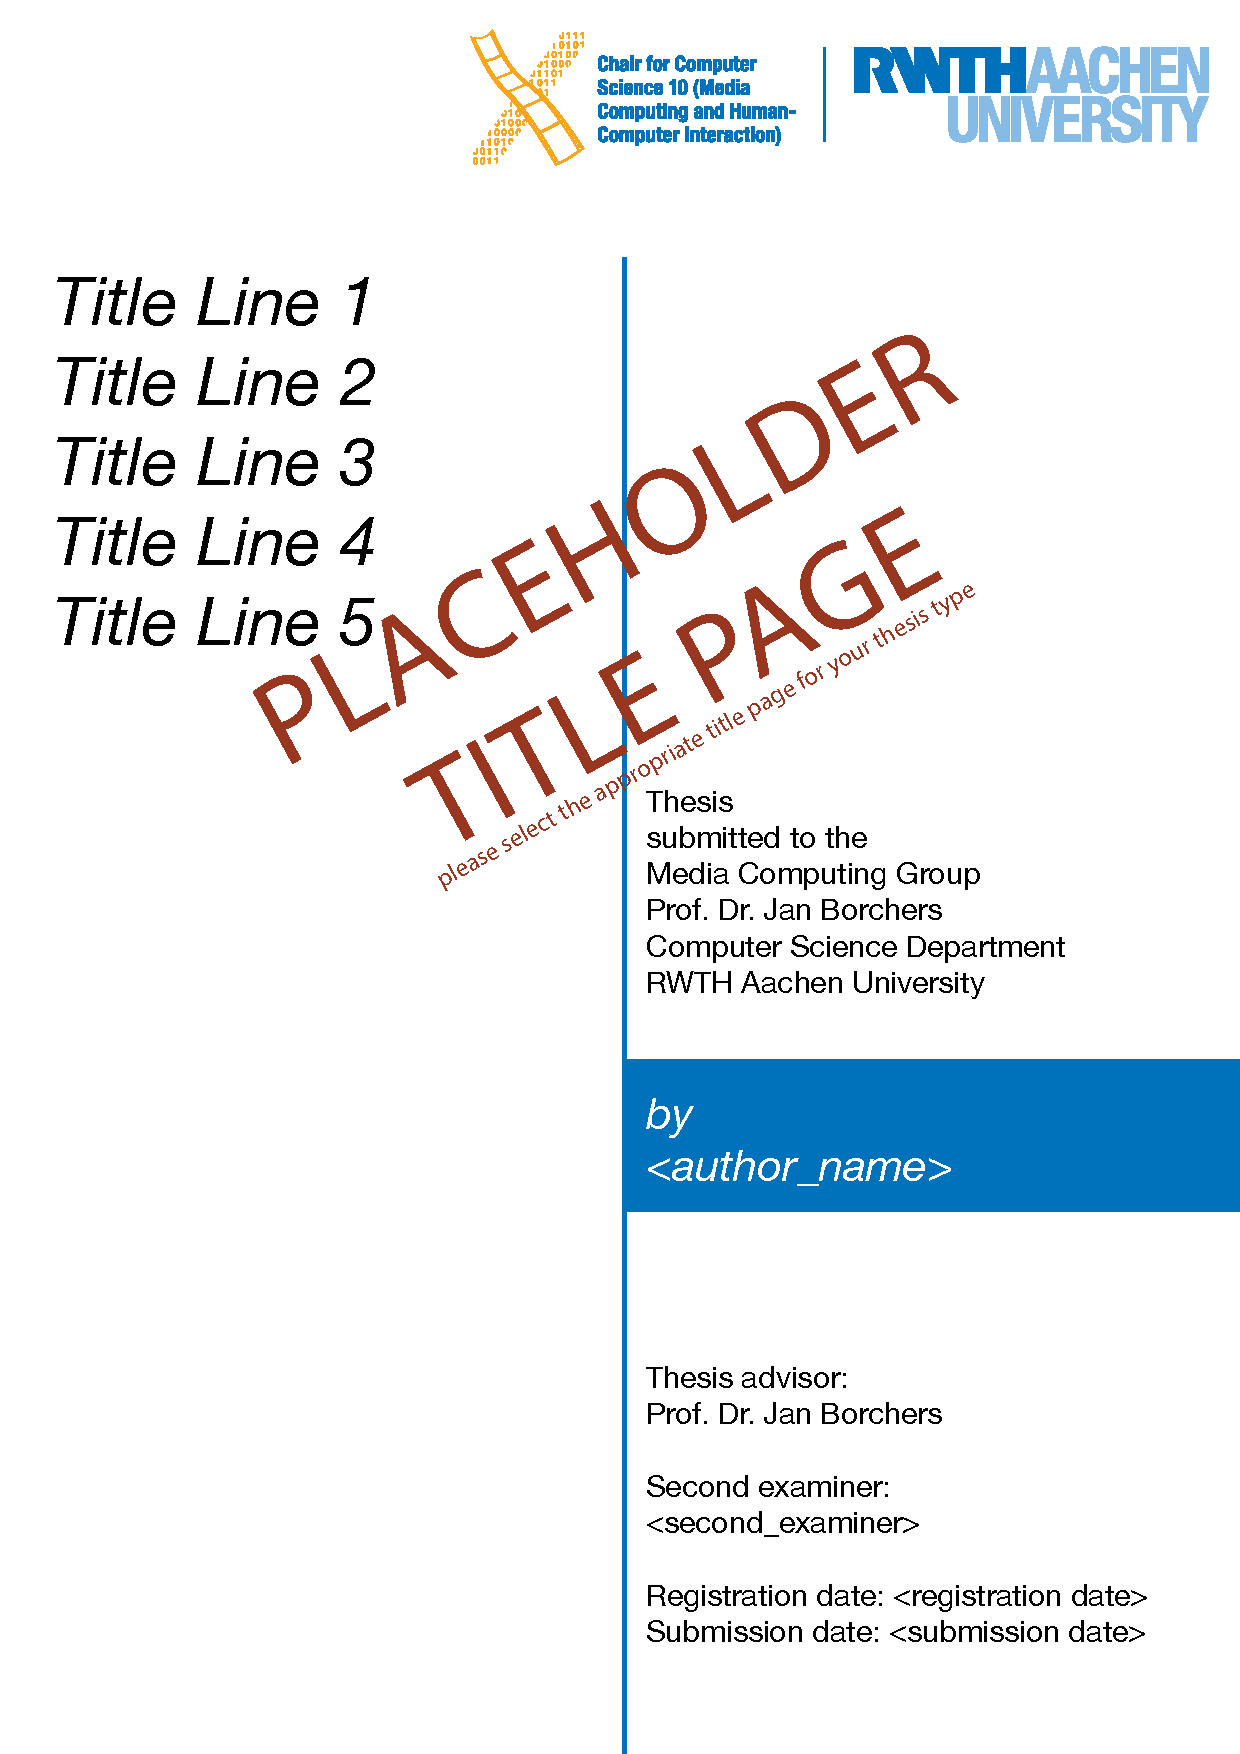
\includegraphics[width=\paperwidth]{titlepage_CID}}}
\strut
\end{titlepage}

\thispagestyle{empty}
\emptydoublepage

% This file is part of the i10 thesis template developed and used by the
% Media Computing Group at RWTH Aachen University.
% The current version of this template can be obtained at
% <http://www.media.informatik.rwth-aachen.de/karrer.html>.

% As of WS2015/16 the ZPA only accepts its own statement of oath: 

\begin{titlepage}
\AddToShipoutPicture*{
\put(0,0){
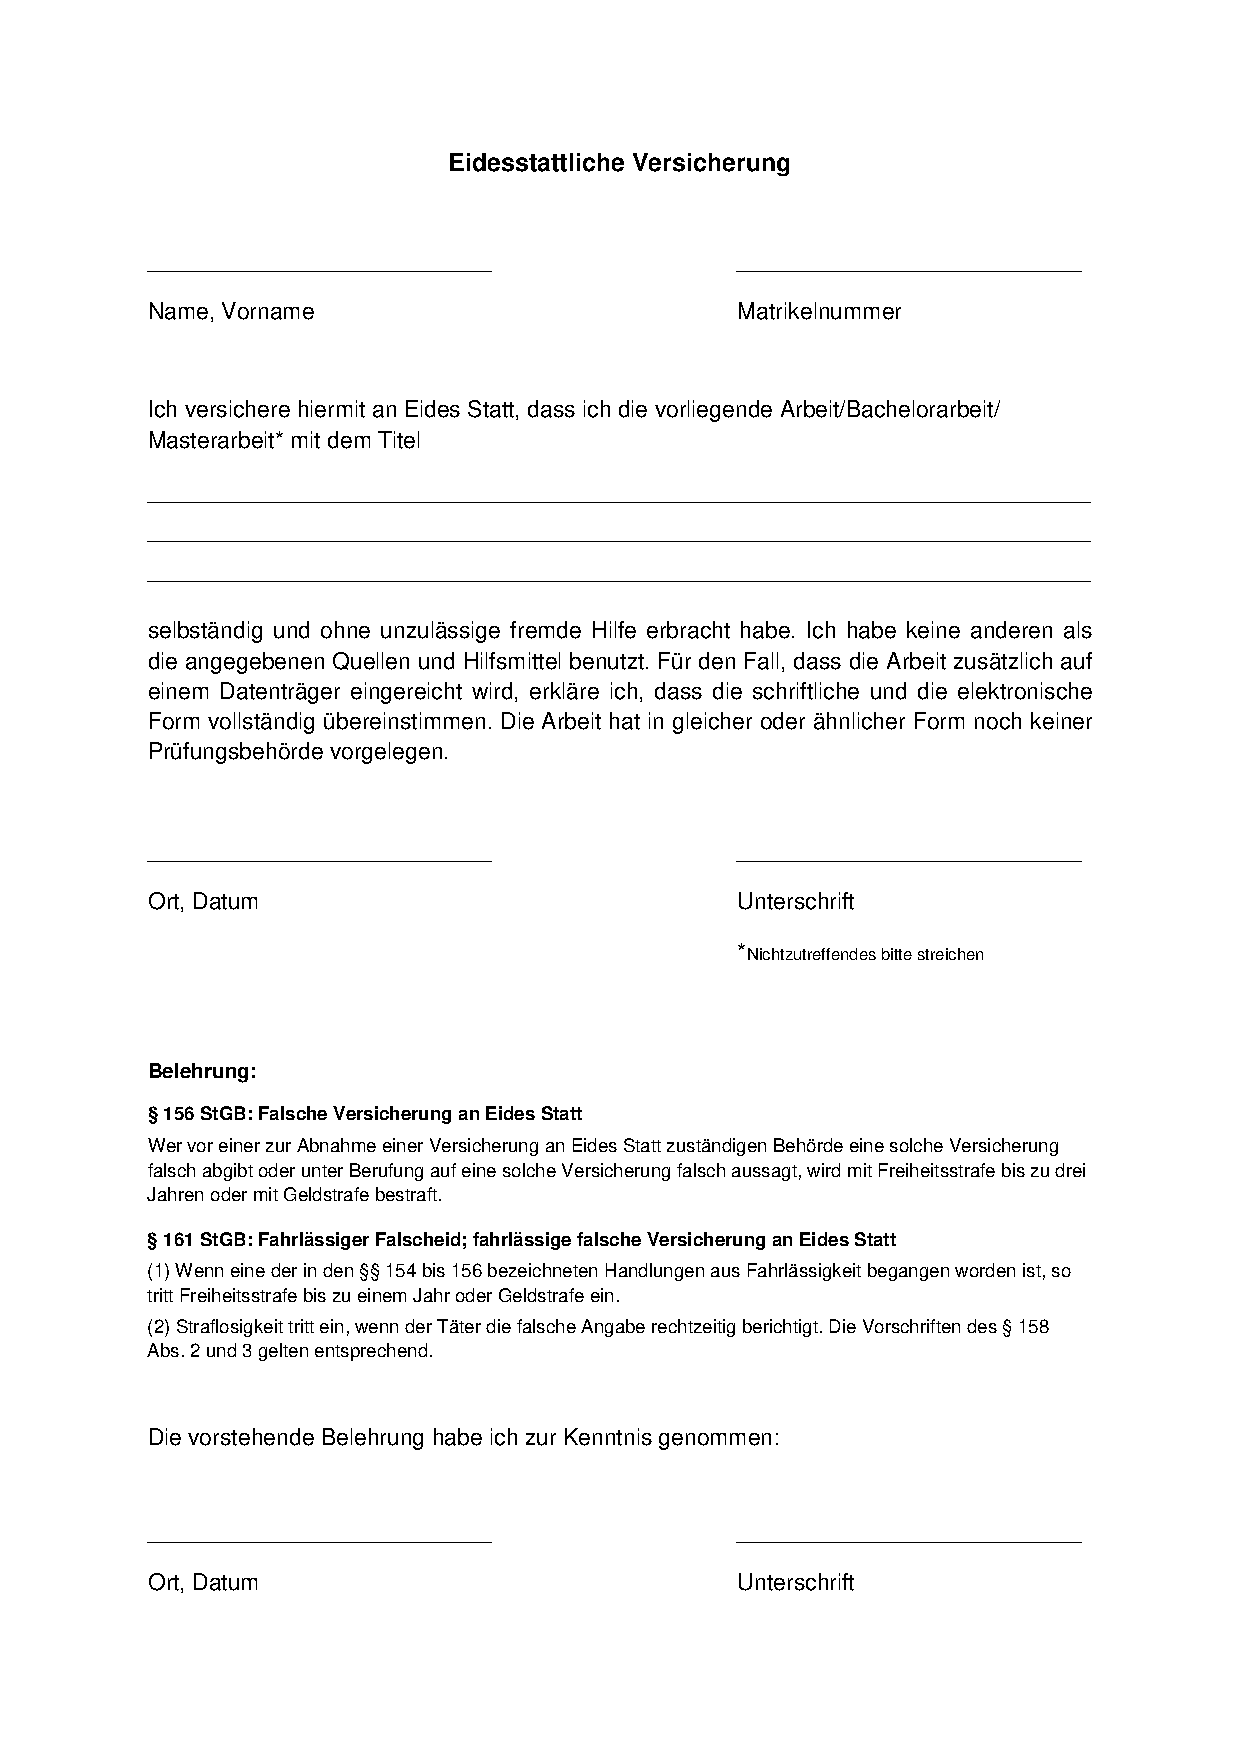
\includegraphics[width=\paperwidth]{oathstatement}}}
\strut
\end{titlepage}

% The following lines are depricated. Only uncomment them when your thesis is _not_ submitted to RWTH Aachen University. In this case, comment the lines 8–13 (above) in addition to remove the ZPA statement of oath.

%~
%\vfill
%I hereby declare that I have created this work completely on my own and used no other sources or tools than the ones listed, and that I have marked any citations accordingly.
%
%Hiermit versichere ich, dass ich die vorliegende Arbeit selbst\"andig verfasst und keine anderen als die angegebenen Quellen und Hilfsmittel benutzt sowie Zitate kenntlich gemacht habe. 
%
%\begin{flushright}
%\vspace{12mm}
%$\overline{Aachen, MONTH \mathit{YEAR}}$\\
%\textit{YOUR NAME}
%\end{flushright}

\emptydoublepage

\setcounter{page}{5}

\tableofcontents
\emptydoublepage
%
\listoffigures
\emptydoublepage
%
\listoftables
\emptydoublepage

%Die �bersicht sollte in englischer und in deutscher Sprache verfasst werden
%the abstract should include an english and a german version
%!TEX root = ./main.tex

% This file is part of the i10 thesis template developed and used by the
% Media Computing Group at RWTH Aachen University.
% The current version of this template can be obtained at
% <http://www.media.informatik.rwth-aachen.de/karrer.html>.

\loadgeometry{myAbstract}

\chapter*{Abstract\markboth{Abstract}{Abstract}}
\addcontentsline{toc}{chapter}{\protect\numberline{}Abstract}
\label{abstract}

%here (english version)
A lot of research is going into underwater global positioning systems. However the few navigation systems out there use bulky screen devices which are held in hand. This leads to constrained movement and is rather obtrusive. In this master thesis we describe the construction of a prototype, which incorporates several feedback methods, and its evaluation. We implement a vibration motor, a LED, and a peltier element in diving goggles and a headband. Since these devices are worn on the head it allows an unintrusive way to give directional cues. We evaluate the feedback methods ashore as a baseline and compare it to their performance underwater. 

\chapter*{\"Uberblick\markboth{\"Uberblick}{\"Uberblick}}
\addcontentsline{toc}{chapter}{\protect\numberline{}\"Uberblick}
\label{ueberblick}

%here (deutsche version)
Lorem ipsum dolor sit amet, consectetur adipisicing elit, sed do eiusmod tempor incididunt ut labore et dolore magna aliqua. Ut enim ad minim veniam, quis nostrud exercitation ullamco laboris nisi ut aliquip ex ea commodo consequat. Duis aute irure dolor in reprehenderit in voluptate velit esse cillum dolore eu fugiat nulla pariatur. Excepteur sint occaecat cupidatat non proident, sunt in culpa qui officia deserunt mollit anim id est laborum.Lorem ipsum dolor sit amet, consectetur adipisicing elit, sed do eiusmod tempor incididunt ut labore et dolore magna aliqua. Ut enim ad minim veniam, quis nostrud exercitation ullamco laboris nisi ut aliquip ex ea commodo consequat. Duis aute irure dolor in reprehenderit in voluptate velit esse cillum dolore eu fugiat nulla pariatur. Excepteur sint occaecat cupidatat non proident, sunt in culpa qui officia deserunt mollit anim id est laborum.Lorem ipsum dolor sit amet, consectetur adipisicing elit, sed do eiusmod tempor incididunt ut labore et dolore magna aliqua. Ut enim ad minim veniam, quis nostrud exercitation ullamco laboris nisi ut aliquip ex ea commodo consequat. Duis aute irure dolor in reprehenderit in voluptate velit esse cillum dolore eu fugiat nulla pariatur. Excepteur sint occaecat cupidatat non proident, sunt in culpa qui officia deserunt mollit anim id est laborum.Lorem ipsum dolor sit amet, consectetur adipisicing elit, sed do eiusmod tempor incididunt ut labore et dolore magna aliqua. Ut enim ad minim veniam, quis nostrud exercitation ullamco laboris nisi ut aliquip ex ea commodo consequat. Duis aute irure dolor in reprehenderit in voluptate velit esse cillum dolore eu fugiat nulla pariatur. Excepteur sint occaecat cupidatat non proident, sunt in culpa qui officia deserunt mollit anim id est laborum.


\loadgeometry{myText}

\emptydoublepage

%Danksagungen
%acknowledgements
%!TEX root = ./main.tex
%
% This file is part of the i10 thesis template developed and used by the
% Media Computing Group at RWTH Aachen University.
% The current version of this template can be obtained at
% <http://www.media.informatik.rwth-aachen.de/karrer.html>.

\loadgeometry{myAbstract}

\chapter*{Acknowledgements\markboth{Acknowledgements}{Acknowledgements}}
\addcontentsline{toc}{chapter}{\protect\numberline{}Acknowledgements}

%Put your acknowledgements in here.
First of all, I would like to thank Prof. Dr. Jan Borchers for supervising my thesis and Dr.-Ing. Ulrik Schroeder for being my second examiner. 
Secondly, I would like to thank Jan Thar for her feedback and guidance. 
Furthermore, thanks to everyone who participated in the time-consuming user study.
\loadgeometry{myText}


\emptydoublepage

%In der Arbeit verwendete Konventionen (Formelsatz, Definitionen, etc.)
%conventions applied in the thesis (AE/BE, definitions, etc.)
%!TEX root = ./main.tex
%
% This file is part of the i10 thesis template developed and used by the
% Media Computing Group at RWTH Aachen University.
% The current version of this template can be obtained at
% <http://www.media.informatik.rwth-aachen.de/karrer.html>.

\chapter*{Conventions\markboth{Conventions}{Conventions}}
\addcontentsline{toc}{chapter}{\protect\numberline{}Conventions}

Throughout this thesis we use the following conventions.



\bigskip

\emph{Text conventions}

Definitions of technical terms or short excursus are set off in coloured boxes.

\myDefBox{Excursus}
{Excursus are detailed discussions of a particular point in a book, usually in an appendix, or digressions in a written text.}

\medskip

Source code and implementation symbols are written in typewriter-style text.

\texttt{myClass}

\medskip

The whole thesis is written in Canadian English.

\medskip

Download links are set off in coloured boxes.

\myDownloadURL{File: myFile}{file_number.file}{file\myUnderscore number.file}

%\pagebreak

%\emph{Formula conventions}




\emptydoublepage

%--------------------------------------------------------------
\mainmatter

%!TEX root = ./main.tex
%
% This file is part of the i10 thesis template developed and used by the
% Media Computing Group at RWTH Aachen University.
% The current version of this template can be obtained at
% <http://www.media.informatik.rwth-aachen.de/karrer.html>.

\chapter{Introduction}
\label{introduction}

Today navigation systems are a natural part of our everyday life.
They are used in vehicles and every smart phone has GPS and map information as well.
GPS uses 29 satellites in the atmosphere where at least four of them are in view from any spot on the earth at any time.
The satellites are synchronized by control stations around the globe using atomic clocks.
The receiver triangulates the position with the distance information of the satellites.
Most of the time this navigation information is conveyed visually by a screen or auditory with precise instructions.

Underwater navigation can be as crucial as it is outside the water.
From novice snorkellers to experienced scuba (self-contained underwater breathing apparatus) divers navigation information can lead to a better experience or is essential for the task.
Novice divers have no knowledge of the area and are not used to the orientation via certain landmarks.
GPS underwater can help to navigate the user to points of interest, save locations to share them later, find back to the start, or view  the route later on the computer. 

GPS underwater is a complex topic since the signals of GPS satellites do not propagate below the water surface.
Current research investigates different approaches to provide GPS underwater not only for divers but submarines and autonomous underwater vehicles (AUV).
A few systems are out there which already use a floating GPS antenna wired to a screen held by the diver \citep{navdive}.
Another system uses an initial GPS position before submerging and switches to inertial sensor measurements while submerged \citep{ariadna}.
Using acoustic waves in analogy to the radio waves of the GPS satellites is locally used in WaterLinked \citep{waterlinked} and researched \citep{Taraldsen_UnderwaterGPS}.

These systems, partly commercially available, focus on their realization of the GPS problem.
All of them use waterproof encapsulated screens and controls which are held by the user all the time.
On one hand, screens are a rich solution and can provide detailed information not only for navigation.
On the other hand it can be tedious to carry a screen device all time, including the wires and high power consumption.
Other solutions which focus more on the interaction part of underwater navigation systems propose augmented reality diving goggles \citep{scubus}.
It is an all in one system which is most likely expensive and not suitable for everyone.

Since underwater GPS is hard to deploy without a proper test environment we decide to focus on the interaction aspect.
Following the concept of ubiquitous computing we aim to make the technology invisible to achieve high acceptance and less distraction \citep{Weiser:1993:CSI:159544.159617}.
Therefore, we focus on low level feedback which can give directional cues using more affordable electronics.

In this thesis we present our prototype comprising an LED, a vibration motor, a Peltier cooling element, and waterproof headphones.
We describe how it is built and what consideration it implies.
Furthermore we conduct a user study with 10 participants testing the system underwater and one participant outside the water for comparison.
We evaluate for the time it takes the participants to perceive the feedback by and ask for qualitative feedback via a questionnaire and comments.

The results show that light, vibration, and sound achieve rather similar reaction times.
Thermal feedback performs poorly underwater and is not even recognized by all participants.
Additionally, the power consumption of the thermoelectric cooler is not reasonable in mobile environments.
Qualitative feedback supports the data of the study that vibration feedback is recommended to convey low level directional cues underwater since it unobtrusive, well recognizable, and comfortable.









%Navigation under water is a tricky and sometimes critical task when diving. 
%So far, characteristics of the diving spot such as current and landmarks available for orientation determine if is suitable for beginners or whether more experience is necessary. 
%For professional divers commercial navigation systems exist, which mostly consists of a (head-up) display giving precise information. 
%These systems allow divers to keep track of their orientation even under difficult conditions, but the technology necessary is complex and expensive, as the omnipresent GPS localization does not work below the water surface. 
%Systems as proposed by Taraldsen et al.~\cite{Taraldsen_UnderwaterGPS} use acoustic beacon systems, other systems use GPS for an initial calibration and rely on a inertial measurement unit (IMU) under water~\cite{Rossi_Performance}.
%For less safety critical situations, e.g., guiding swimmers snorkeling through a scenic reef, less detailed feedback is necessary, and thus, the presentation of the navigation information can be different. 
%In this paper, we investigate which modality is optimal to communicate such minimal cues for underwater navigation.
%The technology added to the snorkel gear should also be minimal to achieve high acceptance and low distraction, fulfilling the vision of non-visible ubiquitous computing~\cite{Weiser:1993:CSI:159544.159617}.
%
%We compared haptic, visual, and acoustic feedback which is well-researched for orientation cues above the surface. 
%We attached vibration motors, thermoelectric coolers for thermal feedback, and LEDs to the snorkel mask, and had the participants of our study wear waterproof earphones (cf.\ Fig.~\ref{fig:figure1}). 
%We measured reaction times and asked for qualitative feedback.
%While light and vibration achieve similar reaction times, vibration was perceived as being more comfortable. 
%Thermal feedback performed poorly as it stayed unnoticed several times. 

\emptydoublepage
%!TEX root = ./main.tex
%
% This file is part of the i10 thesis template developed and used by the
% Media Computing Group at RWTH Aachen University.
% The current version of this template can be obtained at
% <http://www.media.informatik.rwth-aachen.de/karrer.html>.

\chapter{Related work}
\label{relatedwork}

In this chapter we give an overview of related work and research in the the fields of under water navigation systems. 
It is divided into two parts. First it covers existing systems which incorporate position tracking and underwater feedback today and second research regarding several feedback modalities. 

\section{Underwater Navigation Systems}

\mnote{Navimate}
\cite{mckenzie} developed Navimate which uses a floating radio antenna for GPS and an underwater transducers to communicate with a wrist-worn device via acoustic signals. 
The device receives the signals and uses the information of the GPS and the transducers to determine its location and presents the information on the screen. 

\mnote{NavDive}
\cite{Nehowig} built NavDive which uses a floating GPS receiver wired to a mobile receiver held by the diver. 
It shows the direction to previously set locations and positional information in text form. 

\section{Feedback modalities}


\emptydoublepage
%%!TEX root = ./main.tex
%
% This file is part of the i10 thesis template developed and used by the
% Media Computing Group at RWTH Aachen University.
% The current version of this template can be obtained at
% <http://www.media.informatik.rwth-aachen.de/karrer.html>.

\chapter{Hardware Prototype and Software }
\label{ownwork} 


In this chapter we present the construction of the hardware setup and the user study software. 
Furthermore we talk about the technical considerations regarding each component and their feasibility.


\section{System Design}
The aim of this thesis is to investigate the perception of several feedback modalities underwater and their feasibility for low level navigation cues.
We include visual, auditory, and tactile feedback in form of a LED, waterproof in ear headphones,  a vibration motor, and a thermoelectric cooling module.
The prototype has to incorporate these methods as unobtrusive and comfortable as possible in particular when they are  inactive. 
Electronic connections have to be waterproof, undisturbing, and failsafe.
Furthermore all components should be affordable to provide an advantage over commercial solutions.

To investigate the recognition times and comfort of each technique we built a prototype composed of one LED in the diving goggles as well as a waterproof vibration motor and a Peltier cooling module in a stretchable headband.
The headphones are provided separately.

\paragraph{Visual Feedback}

To provide visual low level feedback we use a common red 5mm LED.
An issue regarding luminous light emitted by an LED is its proneness to water reflections.
These reflections change rapidly due to water undulation and exterior lighting.
The color of the surroundings influence it as well.
For example light blue tiles in a swimming pool render a blue LED almost undetectable.
To provide clear recognizable feedback we tested several colors underwater and came to the conclusion that red LED is better recognizable than other common LED colors.

There are several ways to provide feedback with an LED.
Depending on the way it is presented the user might not notice it fast enough if the brightness increases over time.
However, this might be more comfortable than turning on the LED to full brightness instantly.
Therefore we implement both.
First we set the bright from to full brightness immediately.
Second we increase the brightness from 0\% to 100\%  and back to 0\% over 5.1 seconds resulting in a slowly blinking pattern.
We choose this interval arbitrarily after testing several durations.
This can be further investigated but would go beyond the scope of this thesis since we aim to consider several modalities.


\paragraph{Auditory Feedback}

For auditory feedback we choose AGPTEK E11B IPX8 waterproof in-ear headphones.
The headphones are worn separately from the other components and are connected to the operating MacBook Pro.
Like visual feedback, the comfortability of auditory feedback depends on the way it is presented to the user. 
The audio file played should start immediately and be clearly recognizable.
Furthermore the pitch and loudness should be within an appropriate range.
We use the sound of a sonar since it suits the underwater scenario.


\paragraph{Vibration Feedback}

To provide feedback using vibration actuators we choose waterproof 7mm vibration motors.
They are working at 3.3V with 2.45g at 250Hz.
We tried to make smaller vibration motors waterproof.
Using shrinking tubing and epoxy resin adhesive made them waterproof but running them over night underwater let them stop working regardless.
Thus we have to stick to the larger motor.

We handle the vibration feedback similar to the visual feedback and set it to maximum power instantaneously as well as increasing it over time.
Test have shown that it requires a certain amount of voltage to feel a vibration even outside the water.
Therefore we start at 1,18V and increase to 3.3V over 5.4 seconds.


\paragraph{Thermal Feedback}

\todo{describe how peltier works}
For thermal feedback we choose a CUI CP6014 Thermoelectric Module. 
\cite{Peiris_thermoVR} have shown that users prefer cooling over heating.
Cooling also performs better when it comes to recognition time.
Previously we tested heating and cooling effects in water with 21 degrees and cooling was much faster perceivable than heating.
Additionally heating effects were rarely recognizable.
The Peltier module has a maximum voltage of 2.1V and maximum current of 6A.
Therefore we use an external battery combined with a relay to run it.
There are specific circuit boards to control the temperature of thermoelectric cooing elements.
However we considered that running it on full power is sufficient for our purpose since we are interested in the fastest possible reaction times underwater.


\subsection{Hardware Prototype}
\todo{more pictures of prototype creation and the electronics}

As shown in figure~\ref{fig:ledcloseup} the LED is glued to the diving goggles between the silicone and the frame.
There are three reasons to place the LED there.
First, the LED is not in sight or noticeable when turned off and thus unobtrusive.
Second, the light is diffused by the silicone leading to non-dazzling feedback.
Third, the cable routing is easier compared to placing it within the silicone and still make sure no water gets in.

\begin{figure}
	\includegraphics[width= \textwidth]{images/LEDcloseupcut.png}
	\caption{LED insulated and attached between the silicone and frame of the diving goggles using hotglue. }~\label{fig:ledcloseup}
\end{figure}

In addition to the stretchability of the headband it features \todo{length of fastener} a pair of hook and loop fastener as shown in figure~\ref{fig:headbandfastener}.
This enables adjustable, tight, and still comfortable wear of the headband.
The fasteners were sewn to the 40mm wide elastic band using a Bernina 880.

\begin{figure}
	\includegraphics[width= \textwidth]{images/headbandfastener.png}
	\caption{Stretchable headband with hook and loop fastener+ sewn to it. Allows comfortable adjustment on different head froms and sizes.}~\label{fig:headbandfastener}
\end{figure}

To sense the cooling effect of the thermoelectric module it has to be placed directly onto the users skin.
We achieve this by cutting two holes in the elastic band and put the VCC and Ground wires through it. 
Although the edges of the module seem to be uncomfortable, none of the users noticed it at all while it was turned off.
The heat produced by the Peltier element is no issue underwater since the water naturally conducts the heat away.

\begin{figure}
	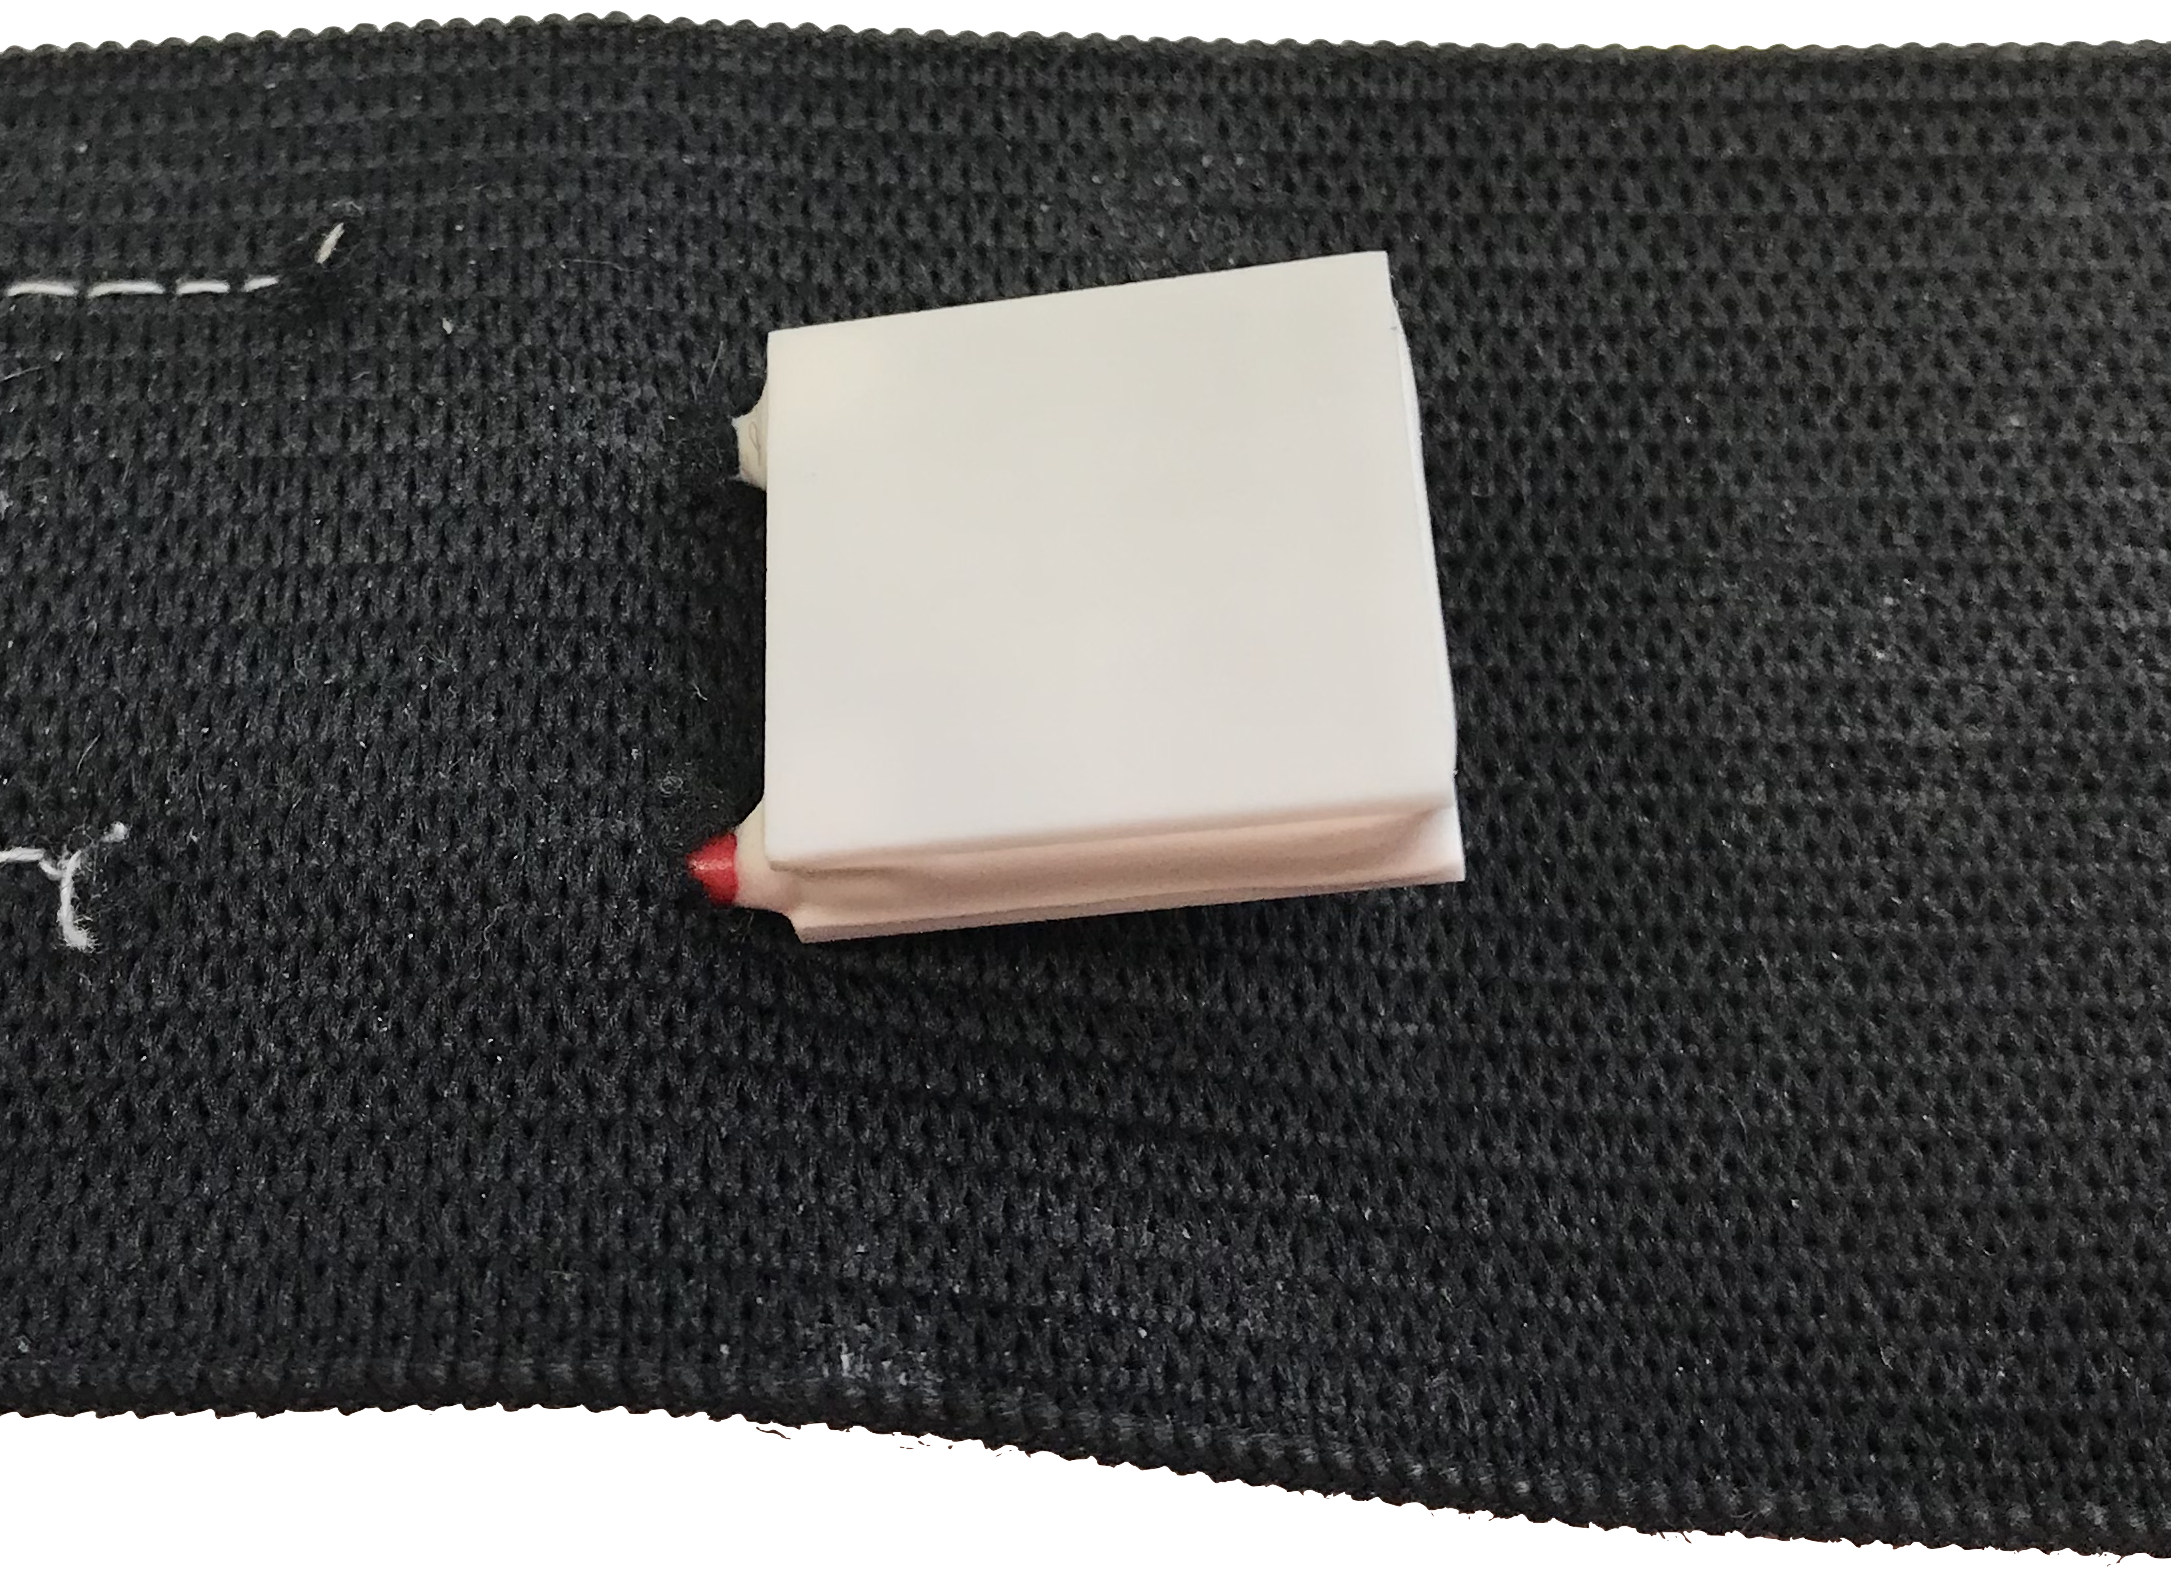
\includegraphics[width= \textwidth]{images/peltier.png}
	\caption{Peltier element mounted to the headband to be placed directly on the users skin.}~\label{fig:peltier}
\end{figure}

As depicted in figure~\ref{fig:headbandmotorbag} a piece of the elastic band was sewn to the headband to house the vibration motor.
Since we choose an already waterproof vibration motor the only challenge is to keep the motor in place and still provide as much tactile performance to the user as possible.
Therefore the the piece of elastic band is sewn to the headband to be at maximum stretch when the motor is in the bag.
The kinetic energy is better transferred by rigid objects.
As for the Peltier element, the motor is not perceived by the user wearing the headband while it is turned off.

\begin{figure}
	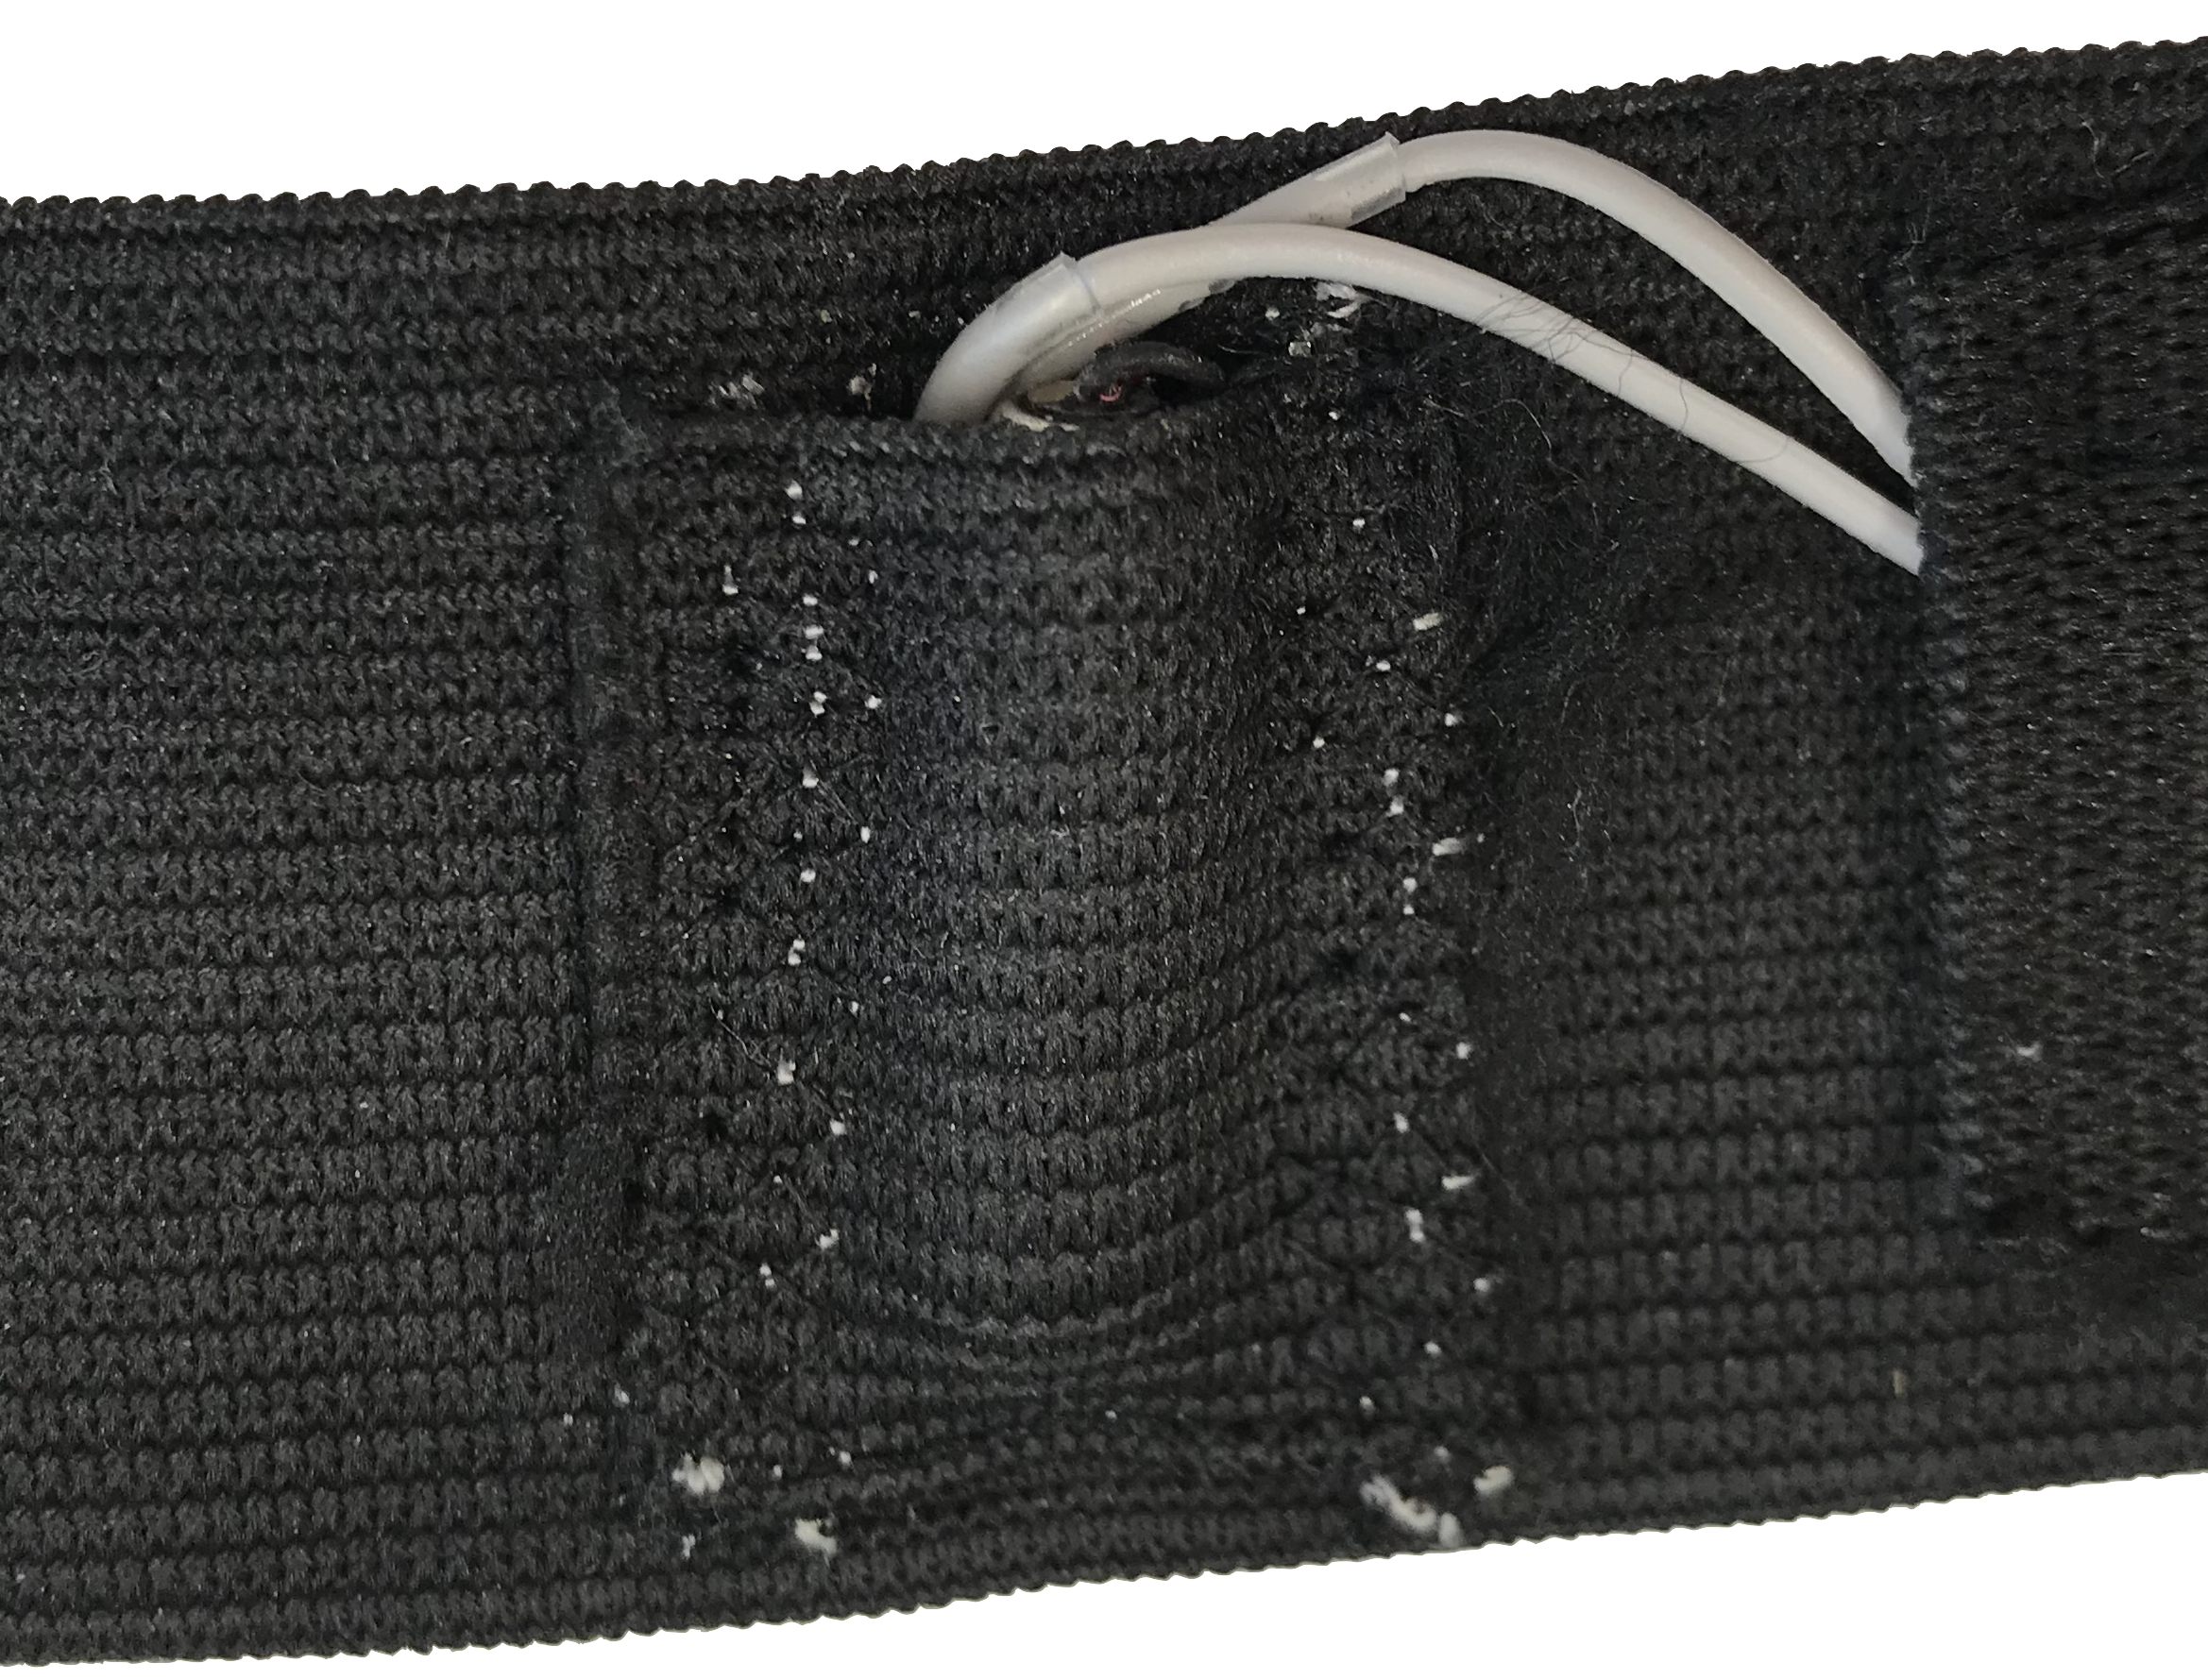
\includegraphics[width= \textwidth]{images/headbandmotorbag.png}
	\caption{Piece of the stretchband sewn to the headband as a bag for the vibration motor.}~\label{fig:headbandmotorbag}
\end{figure}

To prevent the user form tangling up in the wires we sew pieces of the elastic material to the headband as shown in figure \ref{fig:headbandpatches}.
These wireways leading to one side of the headband make wire management easier and prevent them from being damaged.

\begin{figure}
	\includegraphics[width= \textwidth]{images/headbandpatches.png}
	\caption{Pieces of the stretchband sewn to the headband as wireway for better management of the wires.}~\label{fig:headbandpatches}
\end{figure}

The user has to provide feedback if she notices one of the possible kinds of feedback we present to her.
Figure~\ref{fig:button} shows the button we use for that purpose.
We pick a large button used in arcade cabinets and a 3D printed case. 
The button features vertical lift to prevent accidental pressing by the user. 
Furthermore, the supervisor can hear a clearly recognizable click sound when the button was pressed which helps monitoring the functionality of hardware and software.
A consequence of this button design is that the user has to press it outside the water.
This is no issue since the user will stay at the pool edge anyway.

\begin{figure}
	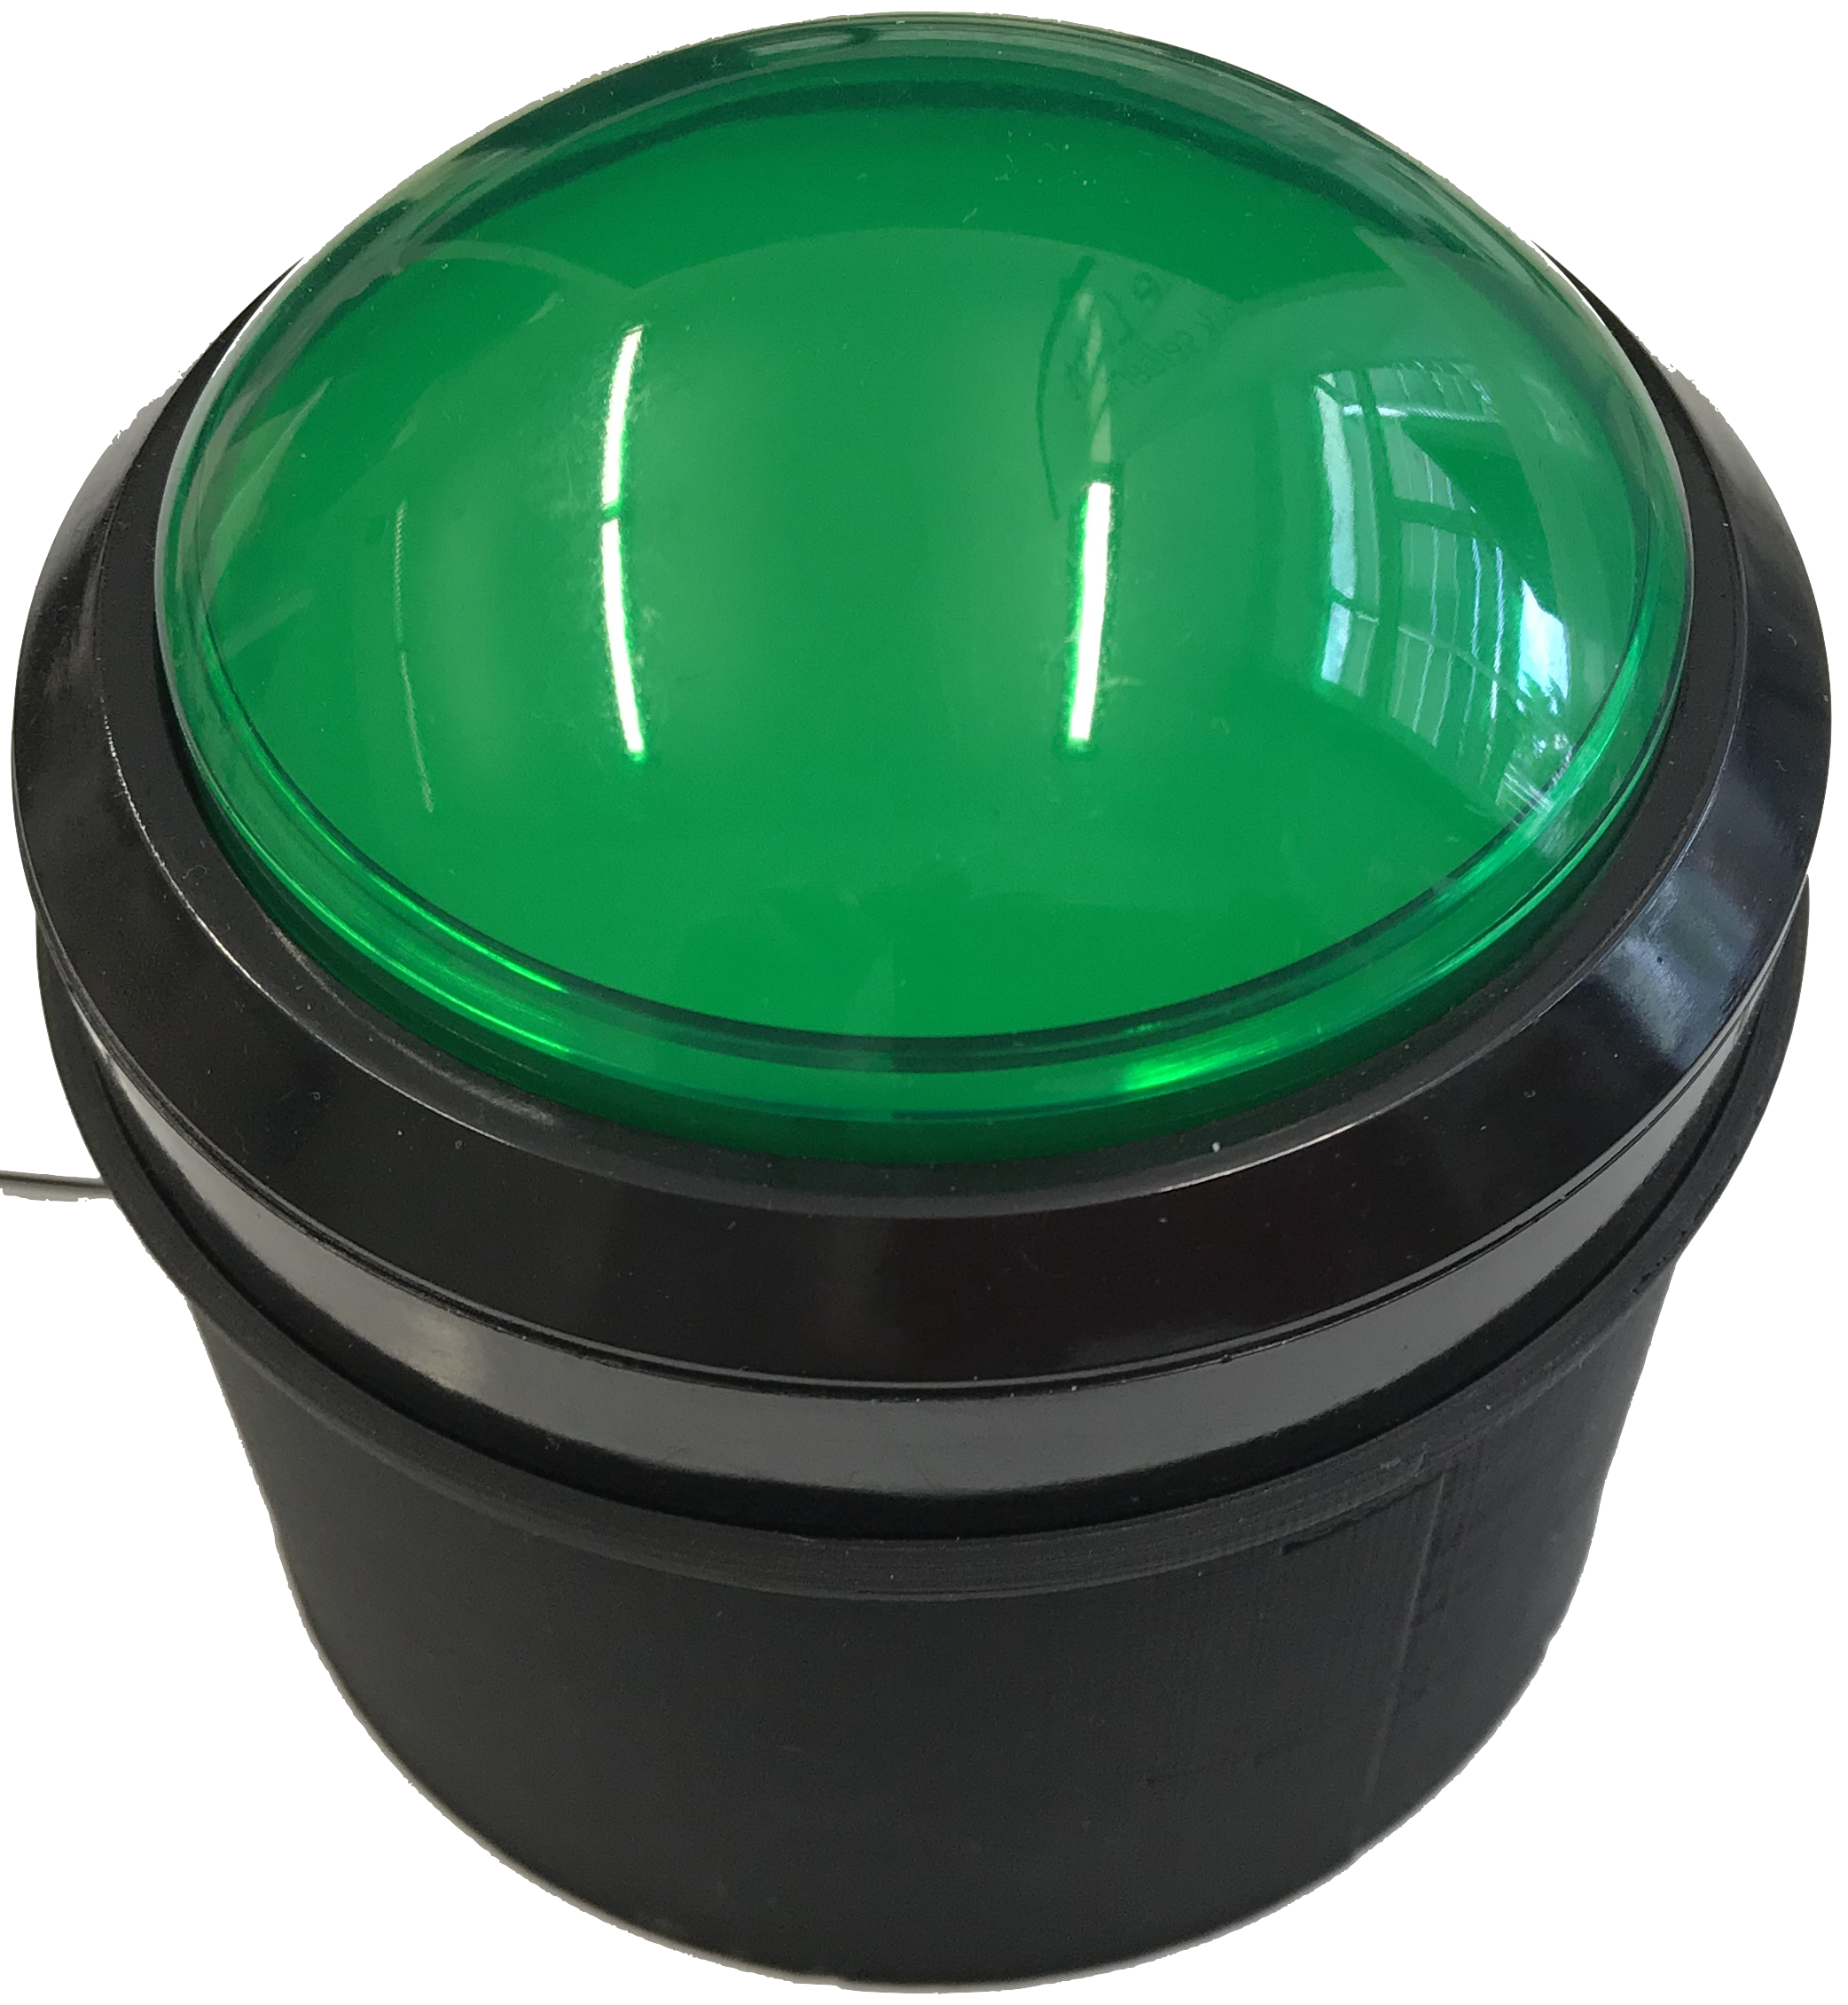
\includegraphics[width= \textwidth]{images/button.png}
	\caption{The botton and the 3D printed case. To be pressed by the user when he recognizes feedback.}~\label{fig:button}
\end{figure}
\todo{length of ribbon cable} 
The wires of the LED, vibration motor, Peltier element, and botton are joined with a ribbon cable depicted in figure~\ref{fig:wires}.
As for all connections and soldering joints, they are made waterproof with glue and shrinking tube.
The ribbon cable leads to the breadboard shown in figure~\ref{fig:breadboard}.
The breadboard houses an Arduino Uno, the cables leading form the pins to the ribbon cable, a relay, and a battery case.
The relay is connected to the Arduino Uno  which controls when it connects the two AA batteries with the Peltier circuit.


\begin{figure}
	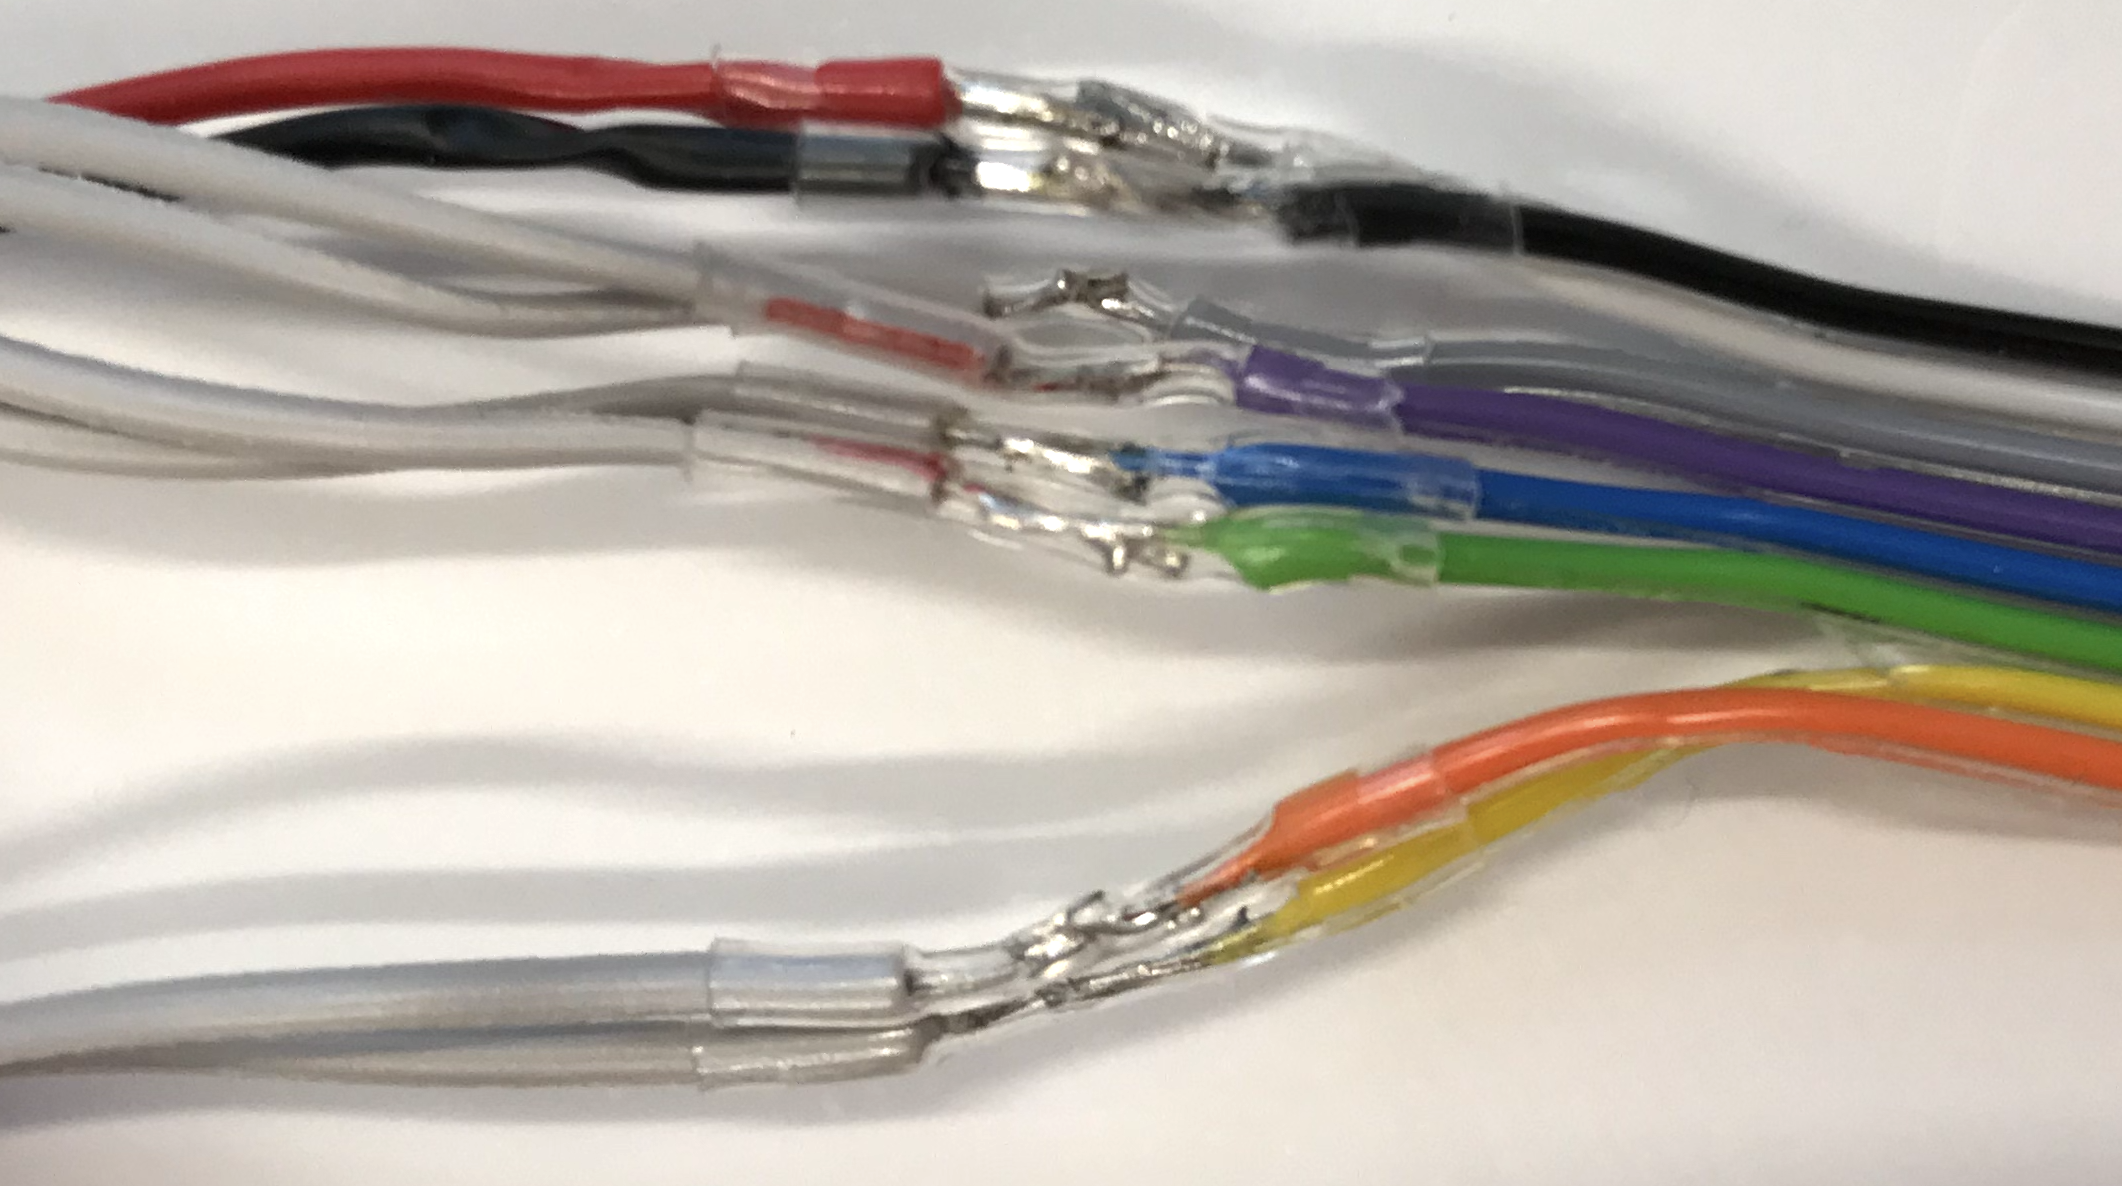
\includegraphics[width= \textwidth]{images/wires.png}
	\caption{Waterproof join of wires from each actuator to the ribbon cable.}~\label{fig:wires}
\end{figure}

\begin{figure}
	\includegraphics[width= \textwidth]{images/breadboard.png}
	\caption{The Arduino controlling the relay and other components of the prototype via the ribbon cable. The batteries power the Peltier element when the relay is set correspondingly.}~\label{fig:breadboard}
\end{figure}


Figure~\ref{fig:studysetupcut} shows all prototype parts worn by the user.
 
\begin{figure}
	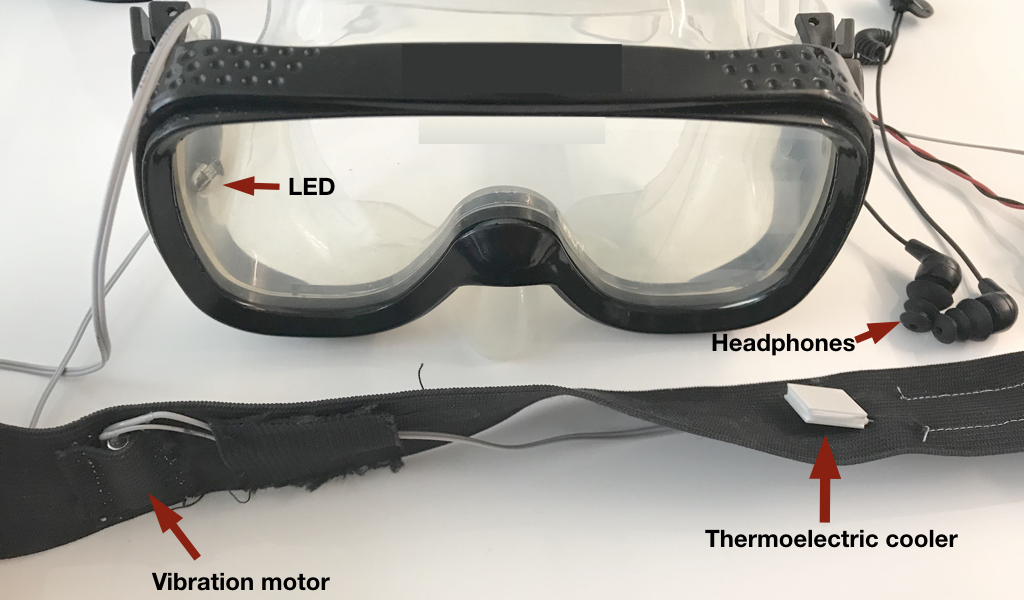
\includegraphics[width= \textwidth]{images/studysetupcut.png}
	\caption{Headband, diving goggles, and waterproof headphones with the integrated LED, Vibration motor, and Thermoelectric cooling module.}~\label{fig:studysetupcut}
\end{figure}


\subsection{Safety}

Since we operate electronics in an underwater test environment, safety concerns arise.
In fact, the voltage and current are below critical values.
Besides, all  wired connections are waterproof and tested for three days in a box filled with water.
The breadboard is always placed in some distance and above the water surface.
During the operation of the prototype in underwater scenario the breadboard and batteries are loosely covered by a towel to protect it against splashing water.

In case the user leaves the pool edge the ribbon cable falls off the breadboard instead of pulling it down. 

\section{Software}

\subsection{Testing}
\emptydoublepage
%!TEX root = ./main.tex
%
% This file is part of the i10 thesis template developed and used by the
% Media Computing Group at RWTH Aachen University.
% The current version of this template can be obtained at
% <http://www.media.informatik.rwth-aachen.de/karrer.html>.

\chapter{Evaluation}
\label{evaluation}
\index{evaluation|(}

In this chapter we will evaluate our prototypes with respect to the quantitative and qualitative aspects of the different feedback methods. We are interested to what extent the perception of feedback differs onshore versus underwater regarding time until the stimulus is perceived. 
We conducted a user study consisting of two parts: in the first part we measured reaction times between presentation of the feedback and it being perceived by the user.
The second part was a questionnaire investigating preferences and experiences regarding the feedback types and their applicability for navigation under water. 
  

\section{User Study}

The apparatus consists of a button at the edge of the pool, diving goggles with an \emph{LED} on the right side, a headband with a vibration motor and a thermoelectric cooler (TEC), and waterproof in-ear headphones. 
These are encapsulated and connected to an Arduino Uno except for the headphones which are directly connected to the MacBook Pro. 
The Arduino measures the time between the activation of a feedback and the press of the button. 
For sound the Arduino sends the command to Processing which then plays the \emph{Sound} file and measures the reaction time. 
Processing logs the time in milliseconds and the corresponding feedback for further analysis.

\subsection{Procedure}

\begin{figure}
	\centering
	\includegraphics[width=\columnwidth]{images/setup2}
	\caption{A participant during the study in a local swimming hall.}~\label{fig:setup2}
	\vspace{-2em}
\end{figure}

The participants took a shower and were asked to swim a few laps until they felt at ease. 
They put on the diving goggles and the headband first, and we ensured that the \emph{peltier element} had direct contact to the skin  of the forehead and that the headband was worn firmly and comfortably. 
Finally, participants put on the snorkel and the earphones. 
Then the participant was instructed to submerge, start the study by pressing the button for the first time, and press the button as soon as she perceives a stimulus.
The prototype is shown in figure~\ref{fig:setup2}. 

Every run included each stimulus eight times in random order with the same stimulus being repeated at most two times in a row. After the button was pressed the next stimulus was randomly delayed between two and eight seconds to prevent adaption. 
This was repeated at least four times per participant with some participants voluntarily doing more runs. 
Participants were allowed to emerge whenever they feel uncomfortable or had issues with the equipment. 
Afterwards, participants answered questions on a 5-point Likert scale regarding feedback recognition, feedback comfort, and imagining the feedback type for underwater navigation.

The equipment is cleaned with sanitizer after usage by participant. 
When acquiring the participants the were allowed to bring their own snorkel if the have hygienic concerns. 

\subsection{Design}
The independent variable was STIMULUS (\emph{simple LED}, \emph{pulsing LED}, vibration, increasing vibration, cooling, \emph{Sound}). 
A sequence of eight stimuli of each type in random order for each run and at least 4 runs per user resulted in (6 x 8 x 4) 192 trials per user in a within-subjects design (48 trials for every additional run). 
The dependent variable is Time [ms] which denoted the time between a stimulus started and the button was pressed.

\subsection{Results}

\begin{figure}
	\centering
	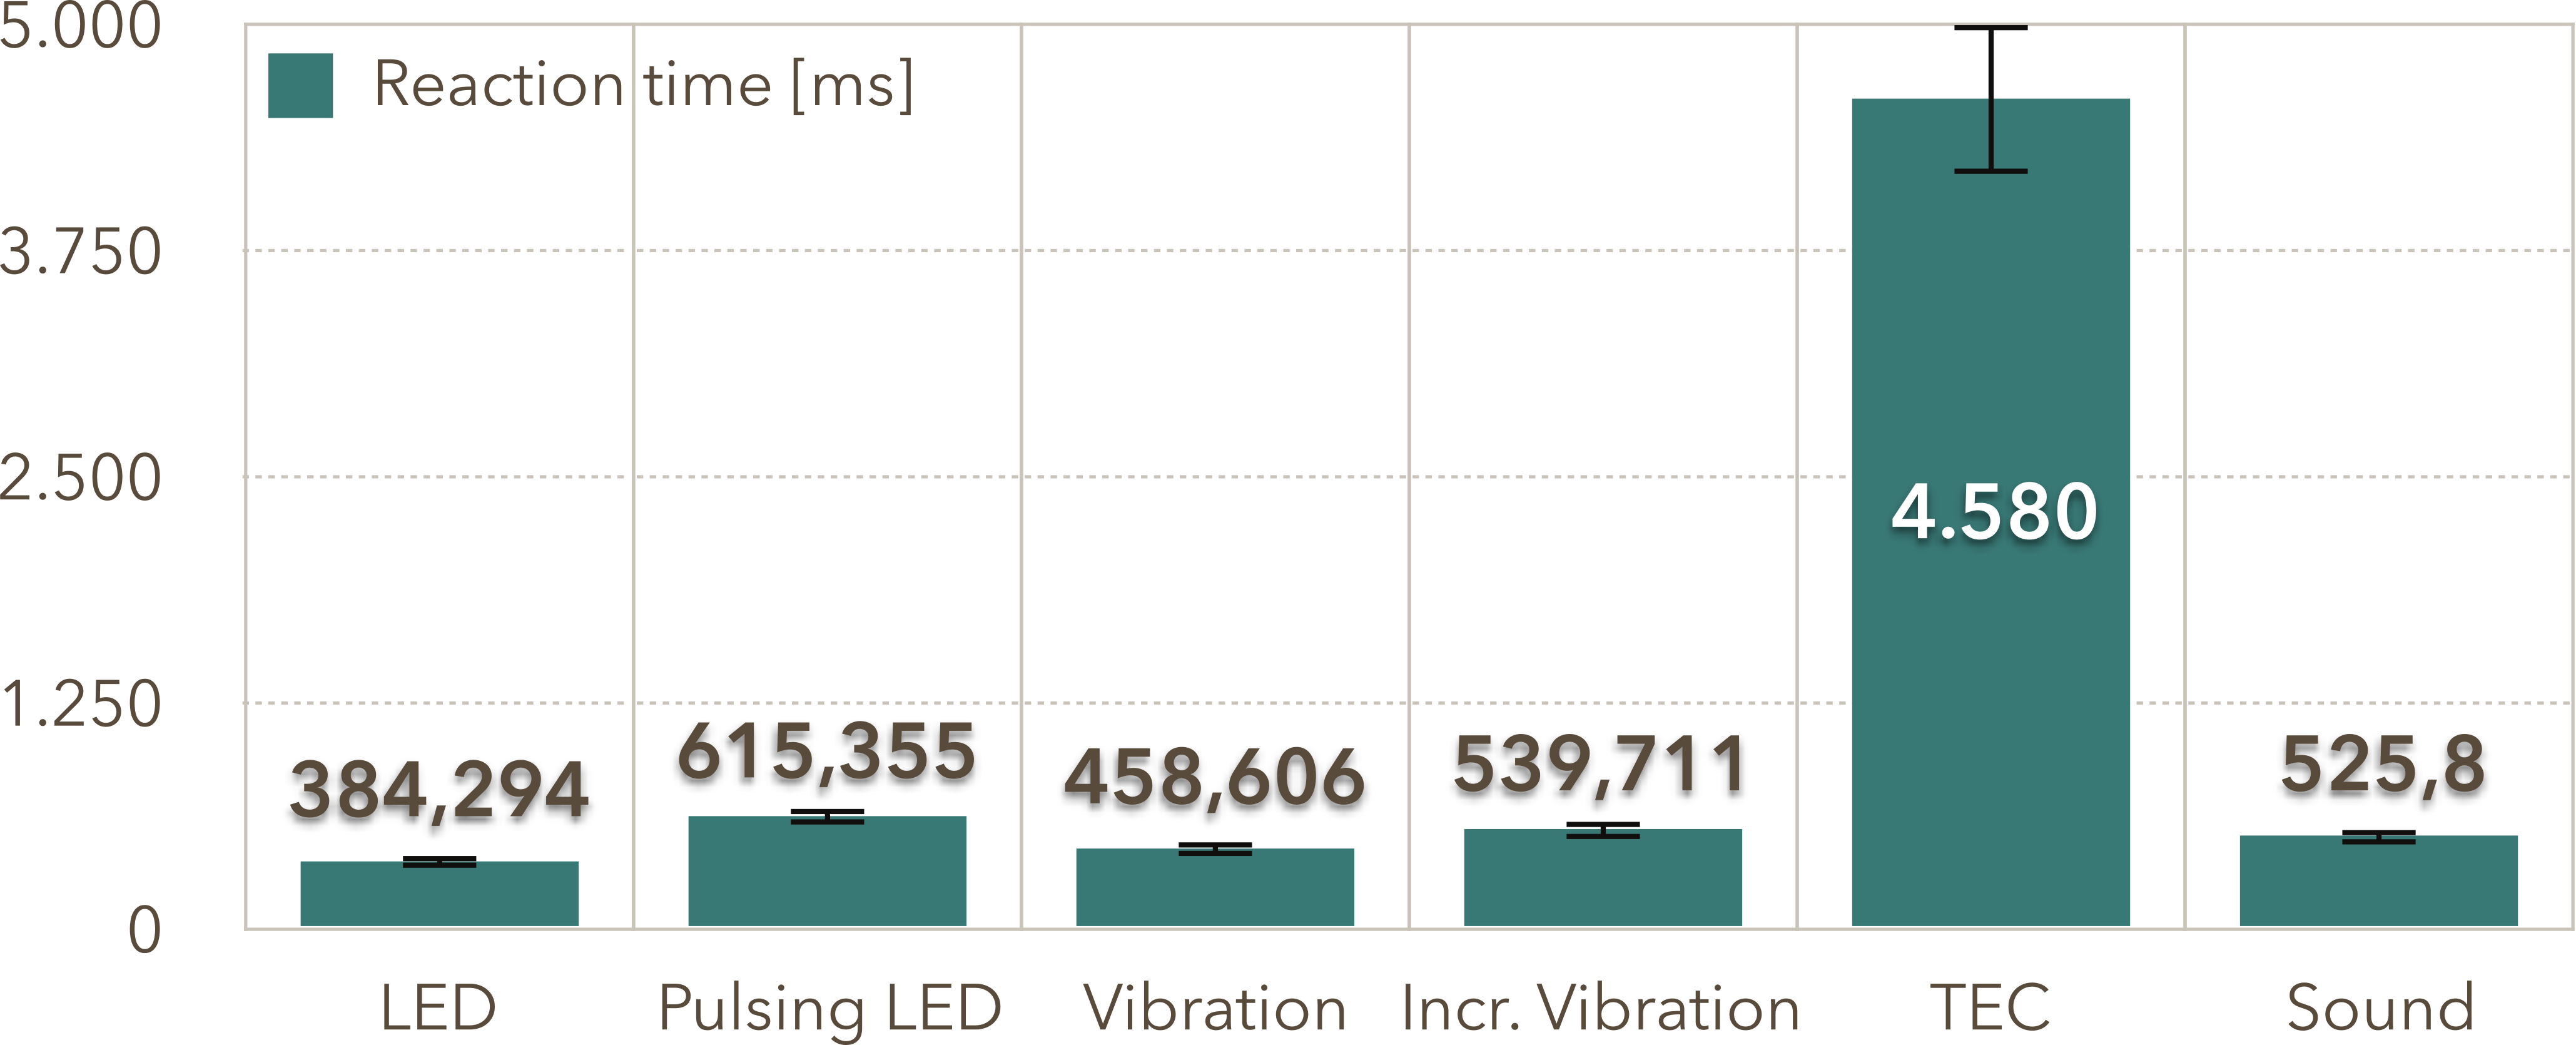
\includegraphics[width=\columnwidth]{images/ResultsOfReactionTimes}
	\caption{Results of the reaction time on different feedback types under water. Means and 95\% confidence intervals.}~\label{fig:reactiontimes}
	\vspace{-2em}
\end{figure}

\begin{figure}
	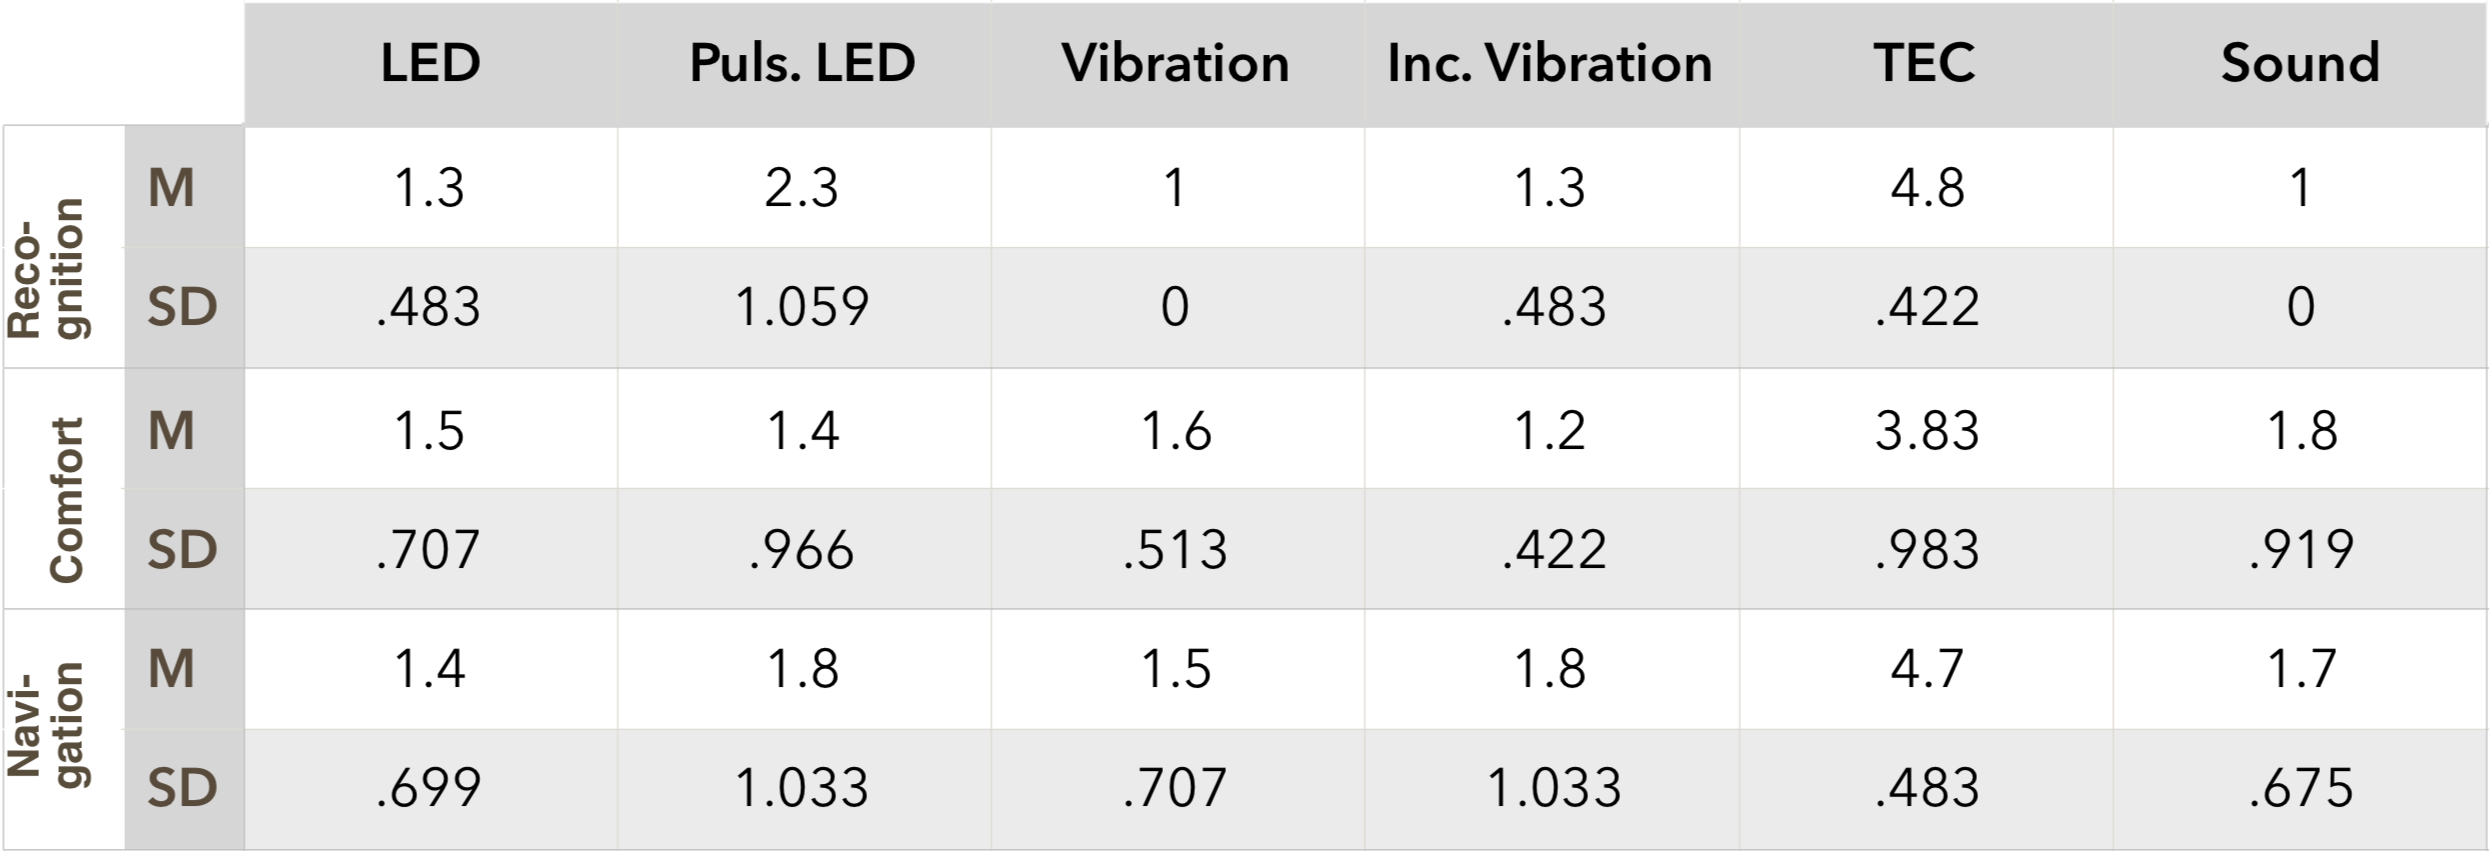
\includegraphics[width=\columnwidth]{images/m_sd_table_noranking}
	\caption{Means and standard deviations (less is better) of the results from the questionnaire.}~\label{fig:m_sd_table}
\end{figure}

\begin{figure}
	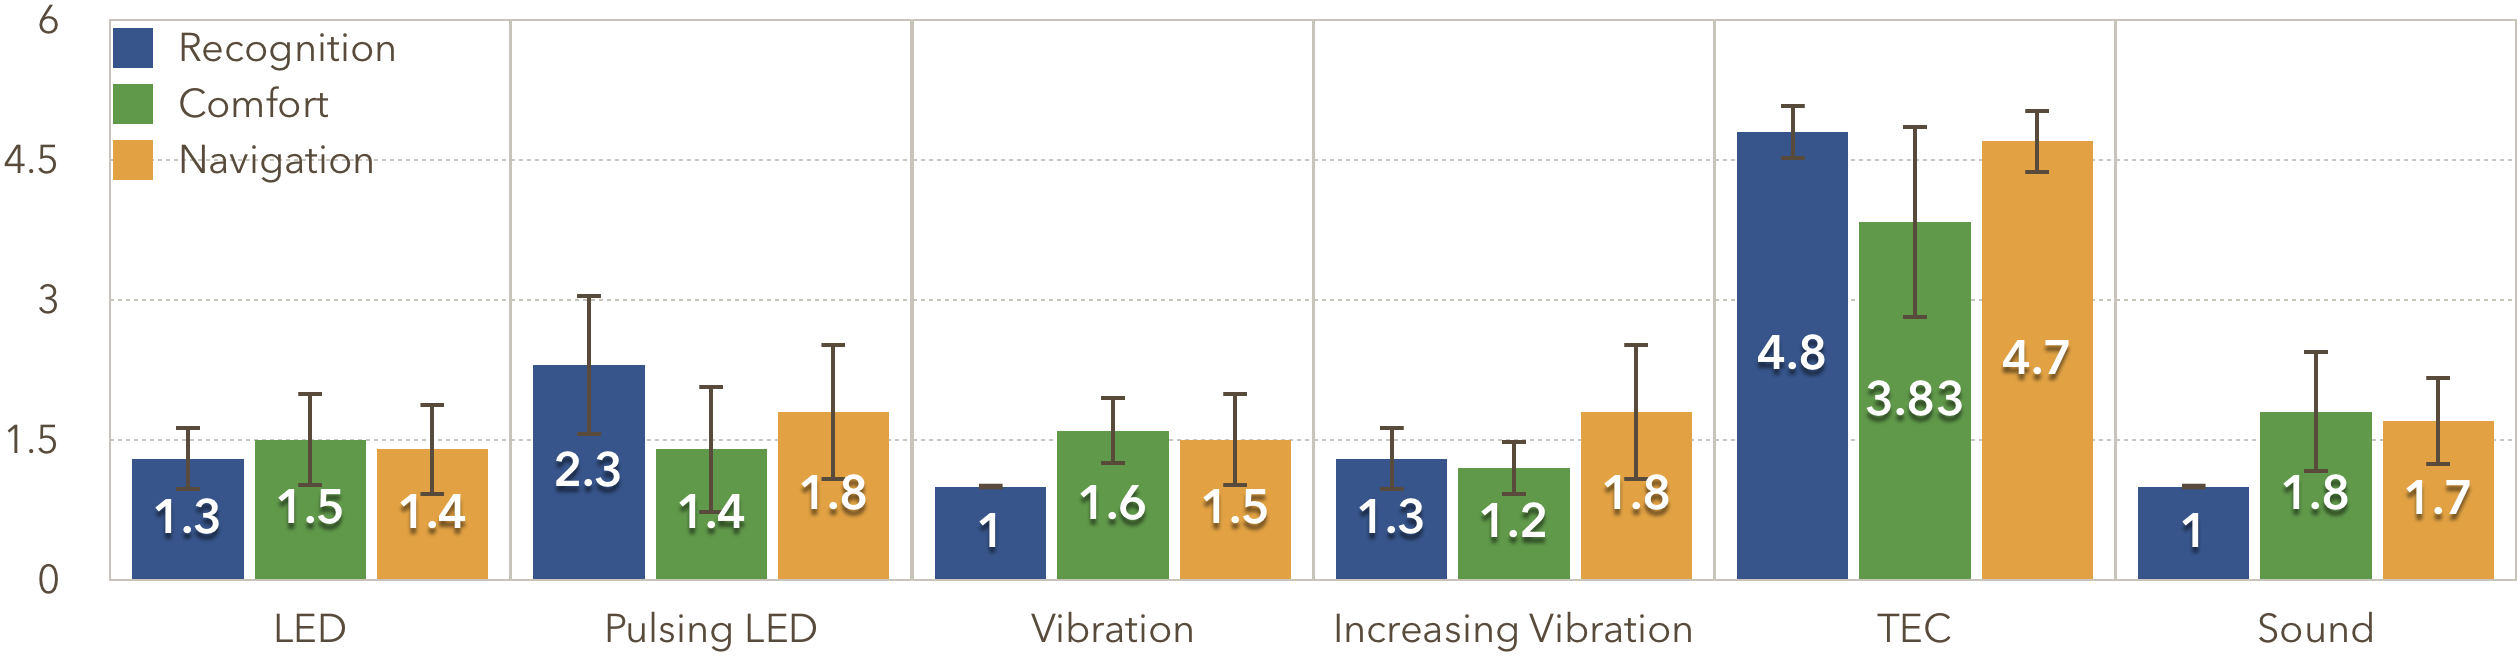
\includegraphics[width=\columnwidth]{images/GraphQuestionnaireNoranking.png}
	\caption{Rating of the feedback modalities by the users (less is better). Means and 95\% confidence intervals of the results from the questionnaire.}~\label{fig:questionnaire}
\end{figure}

A total of 10 users participated in the study (average age 24.1, 8 male), five of which had prior experience with diving or snorkelling. 
391 outliers (results differed by more than 1.5 SD from the mean) were identified resulting in 2021 data points.
The results of the reaction time are shown in figure~\ref{fig:reactiontimes}.
Only 4 participants recognized the \emph{peltier element} at all which \emph{LED} to the majority of outliers. 
The remaining outliers are caused by issues with the equipment (e.g., water in the snorkel or goggles), forcing the participant to emerge.
We log-transformed \emph{Time} for a repeated measures ANOVA. 
{\sc stimulus} had a significant effect on \emph{Time} ($F\textsubscript{1991} = 852.97, p<.0001$). 
Tukey HSD post hoc pairwise comparisons showed that the \emph{peltier element} (4580$ms$) was significantly slower compared to each other {\sc stimulus} and pulsing \emph{LED} (615 $ms$) was significantly slower than vibration (458 $ms$) and simple \emph{LED} (384$ms$).

We used Friedman and Wilcoxon Signed Ranks tests to evaluate the questionnaire (cf.\ Figure~\ref{fig:m_sd_table}).
There was a significant difference in user rated recognition ($\chi^2$(5) = 39.73, $p<.001$).
Post-hoc pairwise comparison revealed that the \emph{peltier element} was perceived significantly less than all other stimuli ($p<.005$). \newline
There was a significant difference in user rated comfort ($\chi^2$(5) = 15.83, $p<.007$).
Post-hoc pairwise comparison revealed that \emph{peltier element} was significantly less comfortable than all other stimuli ($p<.041$) and increasing vibration was significantly more comfortable than vibration ($p<.046$). \newline
There was a significant difference in user rated navigation suitability ($\chi^2$(5) = 28.77, $p<.001$). 
Post-hoc pairwise comparison revealed that only the \emph{peltier element} was rated significantly less suitable for underwater navigation ($p<.004$).

\subsection{Discussion}
The results and the tremendous power consumption show that the \emph{peltier element} is not suitable for underwater applications. 
Participants reported that it is hard to tell whether the \emph{peltier element} is active or if it is a cold flow of water. 
The skin adapts to thermal changes quickly and makes consecutive cooling events hard to detect \citep{Halvey_thermalFeedback}. 

Visual, vibrotactile, and auditory stimuli are suit- able for underwater navigation regarding reaction time (384 - 615 ms). 
Even though the \emph{LED} feedback was fastest (384 ms) the vibration (459 ms) was perceived to be recognized faster. 
Binary feedback using light and vibration is perceived as less comfortable than the fading counterparts. 
Therefore, in an underwater navigation scenario, instant feedback should be used for time critical events only. 
Otherwise, the more comfortable stimuli suffice. 

Participants commented that \emph{LED} feedback can be mistaken for water reflections or to be obstructive and distracting. 
\emph{Sound} was rated as being immediately perceivable (1.0), but some users felt uncomfortable wearing in-ear headphones under water. 
Vibration on the other hand uses a different sense which is not occupied while diving/snorkelling and provides clear and comfortable feedback.
Moreover, the vibration feedback is not influenced by light reflection or water temperature.
Furthermore, vibration feedback acts like bone conductance \emph{Sound}, and therefore, also includes additional auditory feedback.

\subsection{Testing outside the water}

We let one user test it outside the water to get a rough estimate how the medium influences the results in general.
This user is sitting on a table and wears the prototype including the diving goggles but without the snorkel.
The relay we use makes a notable clicking noise which is audible through the headphones worn by the participant.
Therefore we use a pillow and a wastebin to make it infrasonic.
Again we let the user do as many trials as she was willing to do.
210 trials are carried out by the user.
Other than that the procedure and the user study program remain the same as described above.

The results of the participant is shown in figure~\ref{fig:user12}.
It is immediately notable that the visual stimulus is on average faster received in the under water condition (\emph{LED}: 69.285 ms, \emph{Pulsing LED}: 81.708 ms).
Contrarily to the visual modality on average the haptic feedback of the vibration motor is faster perceived outside the water (\emph{Vibration}: 28.822 ms, \emph{Increasing Vibration}: 109.135 ms).
The most preeminent difference between the two mediums is measured when it comes to thermal feedback.
Not only is the cooling effect of the peltier element recognized reliably by the participant, but also 3152.580 ms faster with 1427.657 ms.
\emph{Sound} was perceived negligibly faster underwater with 19.339 ms difference.

\begin{figure}
	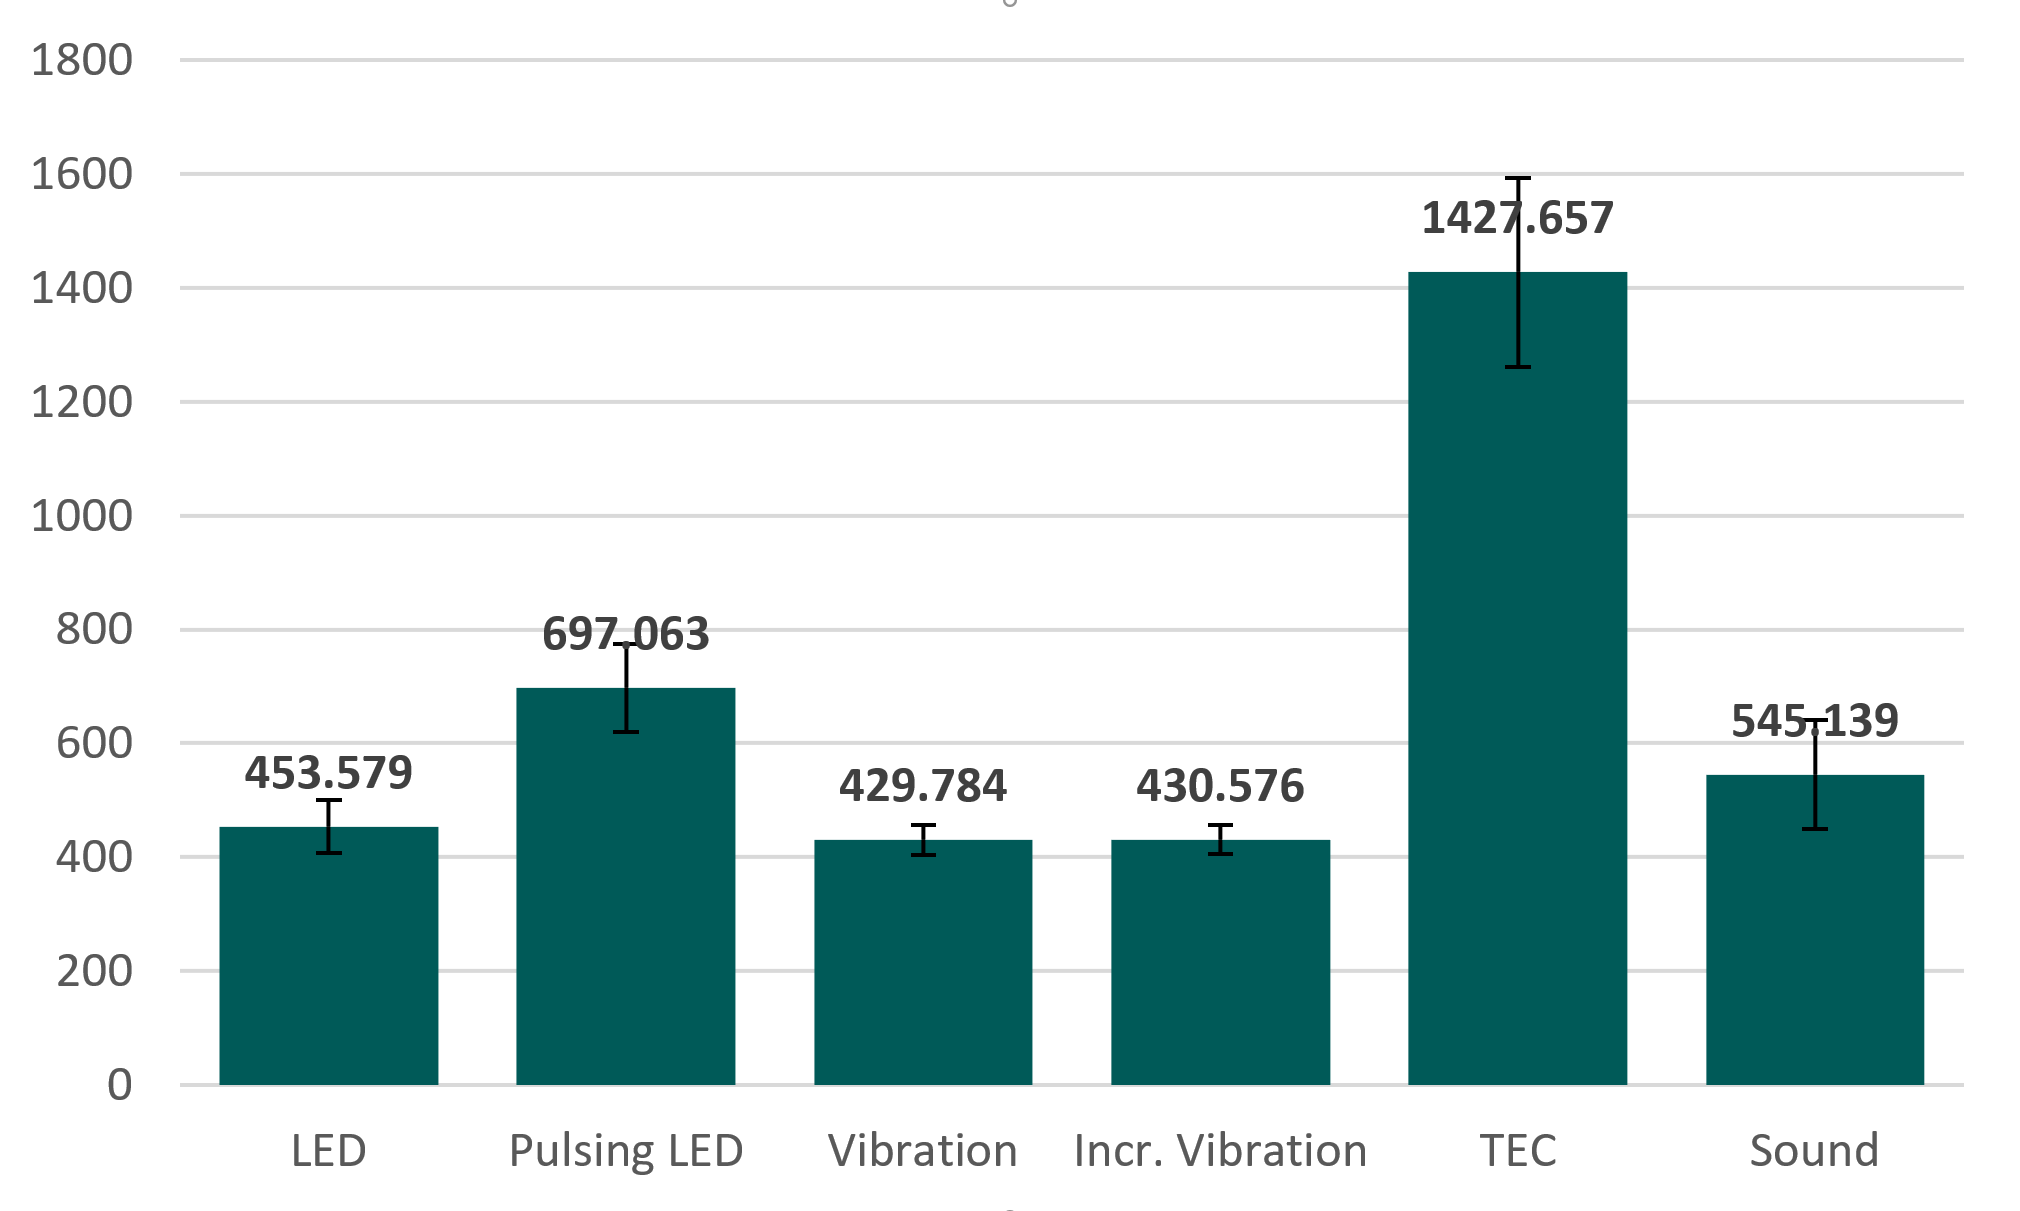
\includegraphics[width=\columnwidth]{images/ResultsOfReactionTimesUser12.png}
	\caption{Results of the reaction time on different feedback types ashore. Means and 95\% confidence intervals. }~\label{fig:user12}
\end{figure}

A reason for the slightly better performance of the \emph{LED} underwater can be explained by the fact that underwater the participants is facing the pool edge where the participant testing the system outside the water has more objects in the room to possibly look at. 
However, the differences for \emph{LED}, \emph{Vibration}, and \emph{Sound} might adjust when testing with more users ashore.
In contrast, the water has a significant influence on the sensibility of the cooling effect provided by the \emph{peltier element}.

\index{evaluation|)}





























\emptydoublepage
%!TEX root = ./main.tex
%
% This file is part of the i10 thesis template developed and used by the
% Media Computing Group at RWTH Aachen University.
% The current version of this template can be obtained at
% <http://www.media.informatik.rwth-aachen.de/karrer.html>.

\chapter{Summary and future work}
\label{summaryandfuturework}

%here

\section{Summary and contributions}
\label{summaryandfuturework.summary}

%here
We built and tested a prototype to investigate the applicability of four feedback modalities for the low-level underwater navigation context.
The prototype consists of diving goggle with a LED glued to it, a stretchable headband with a peltier cooling element and vibration motor, a snorkel, and the electronics including an Arduino Uno.
Visual, tactile, thermal, auditory feedback was investigated for their perceptibility and comfort in underwater scenario.

Results have shown that thermal feedback is not well suited for underwater application since it is not recognizable by a large amount of participants in the first place.
It is heavily influenced by the water and perceivableness varies depending on the water temperature.
This, however, was not observed outside the water where only the technical limitations of the peltier element prolongates the recognition by the user.
Additionally the huge amount of power used by the peltier cooling element makes it impractical to use in mobile environment.

Visual, vibration, and auditory feedback was perceived well and technically suited to provide underwater navigation cues.
Qualitative analysis via a questionnaire, answered by the participants, revealed that vibration feedback performs best on a subjective level.
It does not occupy any of the senses which used for diving in contrast to the LED.
Some user report that wearing the waterproof in-ear headphones is uncomfortable and that they are not used to wear those underwater.

\section{Future work}
\label{summaryandfuturework.futurework}
\index{future work|(}
Our study solely focused on how fast the respective feedback can be perceived underwater and how comfortable it is.
We did not yet investigate how accurate the feedback methods can communicate navigation cues in the field.
In the future we will drop the Peltier element due to its bad performance underwater and massive power consumption.
Furthermore we will tweak our prototype to incorporate a symmetrical amount of LEDs and vibration motors.
The exact amount has to be investigated with a separate user study.

Since the vibration feedback on the head might have an influence on the comfort in the long term, we suggest to implement the vibration motors directly in the diving equipment of scuba-divers.
Well accepted locations were investigated by \cite{Kiss:2018:NSM:3173574.3174191}.

Accuracy of the navigation cues is the most interesting measurement after proving the perceivableness.
To compare the performance of low level cues and more sophisticated approaches, like augmented reality diving goggles and precise auditory instruction via bone conduction headphones, further investigation in real world scenarios will be conducted.

To conduct studies in the field the prototype will be made wireless.
The primary challenges will be the waterproof incorporation of the power supply and electronics as well as establishing precise measurements.
The omission of real time observation and communication requires technology presented in chapter~\ref{relatedwork}.
%here


\index{future work|)}

\emptydoublepage

\begin{appendix}
%!TEX root = ./main.tex
%
% This file is part of the i10 thesis template developed and used by the
% Media Computing Group at RWTH Aachen University.
% The current version of this template can be obtained at
% <http://www.media.informatik.rwth-aachen.de/karrer.html>.

\chapter{TITLE OF THE FIRST APPENDIX}
\label{app.01}

Lorem ipsum dolor sit amet, consectetur adipisicing elit, sed do eiusmod tempor incididunt ut labore et dolore magna aliqua. Ut enim ad minim veniam, quis nostrud exercitation ullamco laboris nisi ut aliquip ex ea commodo consequat. Duis aute irure dolor in reprehenderit in voluptate velit esse cillum dolore eu fugiat nulla pariatur. Excepteur sint occaecat cupidatat non proident, sunt in culpa qui officia deserunt mollit anim id est laborum.Lorem ipsum dolor sit amet, consectetur adipisicing elit, sed do eiusmod tempor incididunt ut labore et dolore magna aliqua. Ut enim ad minim veniam, quis nostrud exercitation ullamco laboris nisi ut aliquip ex ea commodo consequat. Duis aute irure dolor in reprehenderit in voluptate velit esse cillum dolore eu fugiat nulla pariatur. Excepteur sint occaecat cupidatat non proident, sunt in culpa qui officia deserunt mollit anim id est laborum.Lorem ipsum dolor sit amet, consectetur adipisicing elit, sed do eiusmod tempor incididunt ut labore et dolore magna aliqua. Ut enim ad minim veniam, quis nostrud exercitation ullamco laboris nisi ut aliquip ex ea commodo consequat. Duis aute irure dolor in reprehenderit in voluptate velit esse cillum dolore eu fugiat nulla pariatur. Excepteur sint occaecat cupidatat non proident, sunt in culpa qui officia deserunt mollit anim id est laborum.Lorem ipsum dolor sit amet, consectetur adipisicing elit, sed do eiusmod tempor incididunt ut labore et dolore magna aliqua. Ut enim ad minim veniam, quis nostrud exercitation ullamco laboris nisi ut aliquip ex ea commodo consequat. Duis aute irure dolor in reprehenderit in voluptate velit esse cillum dolore eu fugiat nulla pariatur. Excepteur sint occaecat cupidatat non proident, sunt in culpa qui officia deserunt mollit anim id est laborum.

\emptydoublepage
%!TEX root = ./main.tex
%
% This file is part of the i10 thesis template developed and used by the
% Media Computing Group at RWTH Aachen University.
% The current version of this template can be obtained at
% <http://www.media.informatik.rwth-aachen.de/karrer.html>.

\chapter{TITLE OF THE SECOND APPENDIX}
\label{app.02}


\emptydoublepage
\end{appendix}

%--------------------------------------------------------------
\backmatter

%Bibliographie
%bibliography
\clearpage
\phantomsection
\addcontentsline{toc}{chapter}{\protect\numberline{}Bibliography}
\bibliography{thesis}
\emptydoublepage

%Index
%index
\markboth{Index}{Index}
\thispagestyle{plain}
\phantomsection
\addcontentsline{toc}{chapter}{\protect\numberline{}Index}
\printindex

%Satzdatum
%date of typesetting
\newpage
\thispagestyle{empty}
\vspace*{\fill}
\hspace*{\fill}{\tiny Typeset \today}

%--------------------------------------------------------------
\end{document}

